\documentclass[12pt, a4paper]{article}

% ---- Packages -----------------------------------------------
\usepackage[margin=1in]{geometry}
\usepackage[doublespacing]{setspace}
\usepackage{amsmath, amssymb}
\usepackage{booktabs}
\usepackage{tabularx}
\usepackage{graphicx}
\usepackage[labelfont=bf, font=small, justification=justified]{caption}
\usepackage[numbers, compress]{natbib}
\usepackage[colorlinks=true, linkcolor=blue, citecolor=blue, urlcolor=blue]{hyperref}
\usepackage{parskip}
\usepackage{lineno}
\usepackage[T1]{fontenc}

\linenumbers
\modulolinenumbers[5]

% Supplementary figure counter
\newcounter{suppfig}
\renewcommand{\thesuppfig}{S\arabic{suppfig}}

% =============================================================
\begin{document}

% ---- Title page ---------------------------------------------
\begin{titlepage}
\begin{center}
{\Large\bfseries The risk was already there: infectious disease
importation at the 2026 FIFA World Cup}

\vspace{1.5cm}

Jose L. Herrera-Diestra$^{1,*}$, Nyall Jamieson$^{2}$, Mallory J. Harris$^{2,3,4}$, Kaiming Bi$^{5}$, Martial L. Ndeffo-Mbah$^{6}$,  Melissa Zeynep Ertem$^{7}$, Amera Al-Amery$^{8}$

\vspace{0.5cm}

{\small
$^{1}$ Department of Mathematics, Tarleton State University, Stephenville, TX 76402, USA\\
$^{2}$ Department of Integrative Biology, University of Texas at Austin, Austin, TX 78712, USA\\
$^{3}$ Department of Biology, University of Maryland, College Park, MD 20742, USA\\
$^{4}$ University of Maryland Institute for Health Computing, North Bethesda, MD 20852, USA\\
$^{5}$ Department of Management, Policy and Community Health, School of Public Health, The University of Texas Health Science Center at Houston, Houston, TX 77030\\
$^{6}$ Department of Veterinary Integrative Biosciences, College of Veterinary Medicine \& Biomedical Sciences, Texas A\&M University, College Station, TX 77843, USA\\
$^{7}$ Thomas J. Watson College of Engineering, State University of New York at Binghamton, NY, 13850, USA\\
$^{8}$ Department of Computer Information Systems, Jordan University of Science and Technology, Irbid, Jordan\\
$^{*}$ Corresponding author.
E-mail: \href{mailto:jherreradiestra@tarleton.edu}{jherreradiestra@tarleton.edu}
}

\vspace{1cm}

\textbf{Running title:} Importation risk at FIFA World Cup 2026

\vspace{0.5cm}

\textbf{Word count (main text):} $\approx$ 3,500

\textbf{Figures:} 5 main + 8 supplementary

\textbf{Tables:} 1
\end{center}
\end{titlepage}

\newpage

% ---- Abstract -----------------------------------------------
\begin{abstract}
\noindent\textbf{Objectives:}
The 2026 FIFA World Cup will draw an estimated 3.5 million visitors from 48 nations to 11 US host cities. We estimated city-level importation risk for five infectious diseases with propagated uncertainty.   

\medskip
\noindent\textbf{Methods:}
Three nested Poisson models were fitted: a pre-tournament baseline (M1), a World Cup-adjusted model (M2), and a schedule-driven model (M3) allocating fans by match venue. Parameter uncertainty was propagated via 5,000 Monte Carlo draws. A diaspora extension using US Census data estimated co-national network entry probabilities at 11 host cities and 15 non-venue cities.

\medskip
\noindent\textbf{Results:}
Under M3, importation probability exceeded 0.99 for dengue at Miami, New York, and Houston (median $\Lambda = 45.0$, 95\% CI 16.0--92.3) and for malaria at Atlanta and New York. Baseline travel accounted for 86--93\% of importations; the World Cup added only 7--14\% above this pre-existing risk. Dengue diaspora-network entry probability was highest at Dallas (0.43), Houston (0.39), and Los Angeles (0.35); non-host cities exceeded most venue hubs.

\medskip
\noindent\textbf{Conclusions:}
Dengue is the dominant importation risk (Miami, New York, and Houston); malaria dominates at Atlanta and New York. City-level surveillance with targeted diaspora community outreach in host and non-host cities is warranted. The schedule-driven Poisson framework is directly transferable to future mega-events.

\medskip
\noindent\textbf{Keywords:} importation risk; FIFA World Cup 2026; dengue; Poisson model; Monte Carlo uncertainty; diaspora networks
\end{abstract}

\newpage

% =============================================================
\section{Introduction}
% =============================================================

Mass gathering events concentrate infectious disease importation risk by drawing large, diverse international populations into a small number of cities over a short period. The 2026 FIFA World Cup (June 11 -- July 19, 2026) is the first edition with 48 participating nations, played across 16 venues in the United States, Canada, and Mexico. The 11 US host cities --- Atlanta, Boston, Dallas, Houston, Kansas City, Los Angeles, Miami, New York, Philadelphia, San Francisco, and Seattle --- are expected to receive approximately 3.5 million international visitors during the tournament period \citep{NTTO2025}, representing the largest single sporting event in US history. The geographic distribution of all 16 WC2026 stadiums across the three host nations is shown in Supplementary Figure~S4.

Importation risk analyses preceding past FIFA World Cups have taken different approaches depending on the host country's disease ecology. Ahead of the 2014 tournament in Brazil, van Panhuis et al.\ quantified dengue risk for international visitors using travel volumes and local incidence data \citep{vanPanhuis2014}. For Russia 2018, concerns centered on respiratory and vaccine-preventable infections in a temperate host, rather than vector-borne diseases \citep{Pshenichnaya2018}. Qatar 2022 prompted assessments of multiple importation pathways --- including dengue, COVID-19, and emerging pathogens --- in a densely populated host nation receiving visitors from endemic regions \citep{AlTawfiq2022}. However, those analyses typically relied on regional-level travel aggregates, reported point estimates without uncertainty quantification, and did not account for the role of co-national diaspora communities as secondary amplification networks after importation. A concurrent multi-pathogen assessment for WC2026 by Lessler et al.~\cite{Lessler2026}, using the GLEAM-EPIRisk mobility framework, screened 77 pathogens across importation risk, outbreak potential, and economic impact, identifying dengue, malaria, and seasonal respiratory viruses among the priority pathogens of elevated concern. The present study is complementary to that breadth-first screening: rather than covering the full pathogen space, we provide city-specific quantitative importation estimates with propagated parameter uncertainty and an explicit diaspora seeding pathway for the five highest-risk diseases. The current analysis focuses on the group-stage period (June 2026) rather than the full tournament window extending into July, as travel volumes and disease incidence inputs are calibrated to June.

Three methodological gaps motivate this study. First, country-level air travel routing data from the Bureau of Transportation Statistics T-100 program enable city-specific risk stratification at all 11 US venues, including cities with historically limited international surveillance coverage (Atlanta, Kansas City, Seattle). Second, literature ranges for under-reporting correction factors and travel-while-infected probabilities span several-fold; propagating that uncertainty into estimates is essential for honest risk communication. Third, co-national diaspora communities --- whose shared language, cultural spaces, and World Cup watch gatherings make them disproportionately likely to interact with infected travelers from the same country --- represent a transmission pathway invisible to standard Poisson arrival models.

We address these gaps with a three-tier nested Poisson importation model with 5,000-draw Monte Carlo uncertainty for five diseases (dengue, malaria, measles, pertussis, influenza), coupled to a diaspora concentration index derived from US Census Bureau American Community Survey data \citep{Census2026WC, tidycensus}. The approach is fully reproducible using only publicly available data sources, and is designed to be extensible to additional diseases, geographies, and future mass gathering events. Its computational simplicity --- requiring only routine air-travel statistics, published surveillance incidence, and standard statistical software --- means it can serve as a rapidly deployable first-pass risk assessment that public health agencies can adapt without specialized mobility-simulation infrastructure, complementing more comprehensive frameworks where resources permit.

% =============================================================
\section{Methods}
% =============================================================

We quantified importation risk for five infectious diseases (dengue, malaria, measles, pertussis, and influenza) at each of the 11 US FIFA World Cup 2026 host cities during June 2026, using three nested Poisson models that share identical disease data so that differences in results reflect travel volume assumptions only.

\subsection{Travel data}

Country-of-residence (COR) monthly arrivals were obtained from the US Customs and Border Protection I-94 programme \citep{CBP_I94}. City-level routing fractions were derived from BTS T-100 International Segment (Form 41 Traffic) nonstop passenger records for June 2023--2025 \citep{BTS_T100}, computed as the share of each country's US-bound passengers that landed at each venue city, averaged over three years for stability. National Travel and Tourism Office (NTTO) projections provided country-specific 2026 growth factors for the 12 largest US inbound source markets \citep{NTTO2025}.

\subsection{Three nested model tiers}

\textbf{Baseline (M1)} used COR June 2024 arrivals routed by T-100 fractions with no World Cup growth adjustment, representing a pre-tournament counterfactual.

\textbf{WC-adjusted (M2)} applied country-specific growth factors (NTTO projection for top 12 markets; a global World Cup factor of 1.174 for other qualified nations; an empirical background trend factor for non-qualified countries) to project June 2026 arrivals, distributed across cities by T-100 fractions.

\textbf{Schedule-driven (M3)} decomposed travel into a World Cup fan stream --- the marginal increment above background trend, routed proportionally to each team's actual match venues --- and a background stream routed by T-100 fractions. This tier correctly redirects fan travel to Canadian and Mexican venues when teams play there, producing a more realistic US city risk distribution. 

Full mathematical derivations of the projected number of arrivals ($N_{c,v}$) for each model tier, including all intermediate calculations and the formal definition of the routing fractions, are provided in Appendix~A of the Supplementary Material.

\subsection{Disease data and Poisson framework}

For each source country $c$, venue city $v$, and disease $d$, the expected number of infected arrivals is:
\[
  \lambda_{c,v,d}
    = N_{c,v} \;\cdot\; \rho_d \;\cdot\; \frac{C_{c,d}}{P_c}
               \;\cdot\; p_d
\]
where $N_{c,v}$ is projected number of arrivals, $\rho_d$ is the source-country under-reporting correction (corrects for undetected cases in surveillance), $C_{c,d}/P_c$ is the reported per-capita incidence ($P_c$ are 2026 national population estimates \citep{Worldometers2026pop}), and $p_d$ is the probability that an infected individual presents with mild or no symptoms and therefore remains travel-capable (severely symptomatic individuals are assumed to opt out of international travel). City-level intensity and importation probability follow as $\Lambda_{v,d} = \sum_c \lambda_{c,v,d}$ and $P(\geq 1)_{v,d} = 1 - e^{-\Lambda_{v,d}}$, where $X_{v,d} \sim \mathrm{Poisson}(\Lambda_{v,d})$ is the number of imported cases at city $v$ for disease $d$; for brevity we write this as $P(\geq 1)_{v,d}$.

Disease-specific incidence was sourced from: WHO Global Dengue Surveillance dataset (monthly; June 2024--2025 average) \citep{WHO_dengue}; WHO World Malaria Report 2024 (annual incidence per 1,000 population) \citep{whoWMR2024}; WHO Immunization Data (annual incidence per million for measles and pertussis) \citep{WHO_immunization}; WHO FluNet GISRS (weekly positive specimens, ISO weeks 22--26, 2023--2025 average). Literature-derived disease parameters are summarised in Table~\ref{tab:params}.

\begin{table}[htbp]
\centering
\caption{Disease parameters and Monte Carlo uncertainty bounds used in all three model tiers. For each of 5,000 iterations, $\rho_d \sim \mathrm{Uniform}(\rho_{\min},\rho_{\max})$ and $p_d \sim \mathrm{Uniform}(p_{\min},p_{\max})$ are drawn independently. All reported estimates are Monte Carlo medians with 95\% uncertainty intervals. Dengue and influenza incidence are June-month values; malaria, measles, and pertussis use annual rates divided by 12 to approximate June incidence.}
\label{tab:params}
\small
\setlength{\tabcolsep}{6pt}
\begin{tabular}{l rr rr l}
\toprule
&
  \multicolumn{2}{c}{$\boldsymbol{\rho_d}$} &
  \multicolumn{2}{c}{$\boldsymbol{p_d}$} & \\
\cmidrule(lr){2-3}\cmidrule(lr){4-5}
\textbf{Disease} &
  \textbf{min} & \textbf{max} &
  \textbf{min} & \textbf{max} &
  \textbf{References} \\
\midrule
Dengue    & 0.06 & 0.26 & 0.30 & 0.70 & \citep{Bhatt2013,undurraga2013} \\[3pt]
Malaria   & 0.10 & 0.35 & 0.10 & 0.50 & \citep{whoWMR2024,lindblade2013,topazian2020} \\[3pt]
Measles   & 0.40 & 0.80 & 0.02 & 0.10 & \citep{simons2012,whittle1999,helfand1998} \\[3pt]
Pertussis & 0.01 & 0.10 & 0.50 & 0.90 & \citep{chen2016,craig2020,althouse2015} \\[3pt]
Influenza & 0.01 & 0.10 & 0.30 & 0.70 & \citep{mccarthy2020,hayward2014,carrat2008,leung2015} \\
\bottomrule
\end{tabular}
\end{table}

\subsection{Monte Carlo uncertainty quantification}

The under-reporting correction $\rho_d$ and travel-while-infected probability $p_d$ each have wide literature ranges reflecting heterogeneity across surveillance systems and epidemiological settings. We treated both as independent Uniform random variables within their literature bounds (Table~\ref{tab:params}) and drew 5,000 samples per disease. For each draw, all city-level $\Lambda_{v,d}$ values were recomputed. Reported estimates are Monte Carlo medians with 95\% uncertainty intervals (2.5th--97.5th percentiles). Because $\rho_d$ and $p_d$ enter multiplicatively, uncertainty intervals are asymmetric. For dengue, the reference $\rho_d$ lies near the lower literature bound, producing strongly right-skewed intervals that indicate the reported estimate is conservative; for pertussis, the reference $\rho_d$ equals the upper bound, producing left-skewed intervals (Supplementary Figure~S3).


\subsection{Diaspora network extension}

Standard Poisson models treat all arrivals identically regardless of the social environment they enter. We extended the framework to estimate the probability that imported cases reach co-national diaspora networks at each host city.

Diaspora concentration was computed from US Census Bureau American Community Survey 5-year estimates (2019--2023), Table B05006, via the \texttt{tidycensus} R package \citep{tidycensus,Census2026WC}, defined as the share of each metro area's total foreign-born population born in each source country.

\textbf{Mechanism A (local social mixing).} Each infected arrival independently contacts the co-national community with a probability proportional to the diaspora concentration index. This yields a city-level probability that at least one imported case enters a co-national network, directly comparable to the main model's $P(\geq 1)$ metric.

\textbf{Mechanism B (return seeding).} US diaspora members may travel domestically to match venues and carry infection back to their home city. A secondary seeding index ranks candidate hub cities by their exposure potential, combining the importation intensity at the match venue with the diaspora concentration in the hub city. Hub cities comprise both the 11 host metropolitan areas and 15 major non-host metropolitan areas with large immigrant populations, drawn from the same ACS country-of-birth data, so that risk returning to non-venue cities is captured.

Full mathematical derivations of both mechanisms and the formal relationship between the diaspora-adjusted and standard importation probabilities, are provided in Appendix~B of the Supplementary Material.

All analyses were conducted in R (version 4.4) using packages \texttt{tidyverse}, \texttt{readxl}, \texttt{cowplot}, and \texttt{tidycensus}.

% =============================================================
\section{Results}
% =============================================================

Unless otherwise noted, results below refer to the schedule-driven  model (M3), which allocates World Cup fan travel by match schedule and is the most faithful representation of actual visitor flows; a direct comparison across all three model tiers is provided in Section~\ref{sec:comparison}.

\subsection{Importation risk by disease and host city}

%    the probability of at least one dengue importation exceeded 99%

Under the schedule-driven model (M3), the probability of at least one dengue importation exceeded 99\% in Miami, New York, and Houston (Figure~\ref{fig:heatmap}; equivalent heatmaps for the Baseline (M1) and WC-adjusted (M2) models are shown in Supplementary Figures~S1 and S2). Miami had the highest absolute importation intensity ($\Lambda = 15.8$, 95\% CI 5.6--32.3), followed by New York (10.5, 95\% CI 3.7--21.5) and Houston (5.6, 95\% CI 2.0--11.4). The dengue importation probabilities exceeded 0.95 in Dallas and Atlanta, while smaller venues --- Boston, Seattle, and Kansas City --- showed substantially lower probabilities. Dengue importation intensity in 11 cities under M3 was 45.0 (95\% CI 16.0--92.3). Malaria risk exceeded $P(\geq 1)>0.99$ in Atlanta and New York, with Atlanta carrying the highest absolute intensity ($\Lambda=8.54$), reflecting the concentration of Sub-Saharan African air routes through Hartsfield-Jackson airport; malaria importation intensity in the 11 cities was 16.4 (95\% CI 4.9--39.1). Pertussis ($\Lambda = 2.0$, 95\% CI 0.5––4.2) and influenza ($\Lambda = 1.8$, 95\% CI 0.4––4.0) showed intermediate importation intensities. Measles had near-zero expected importation intensity ($\Lambda = 0.05$, 95\% CI 0.02--0.10) because WHO-reported per-capita incidence is very low across most World Cup source countries; US measles cases arise primarily from outbreak chains seeded by a small number of imports rather than a large number of imported cases.

\begin{figure}[htbp]
  \centering
  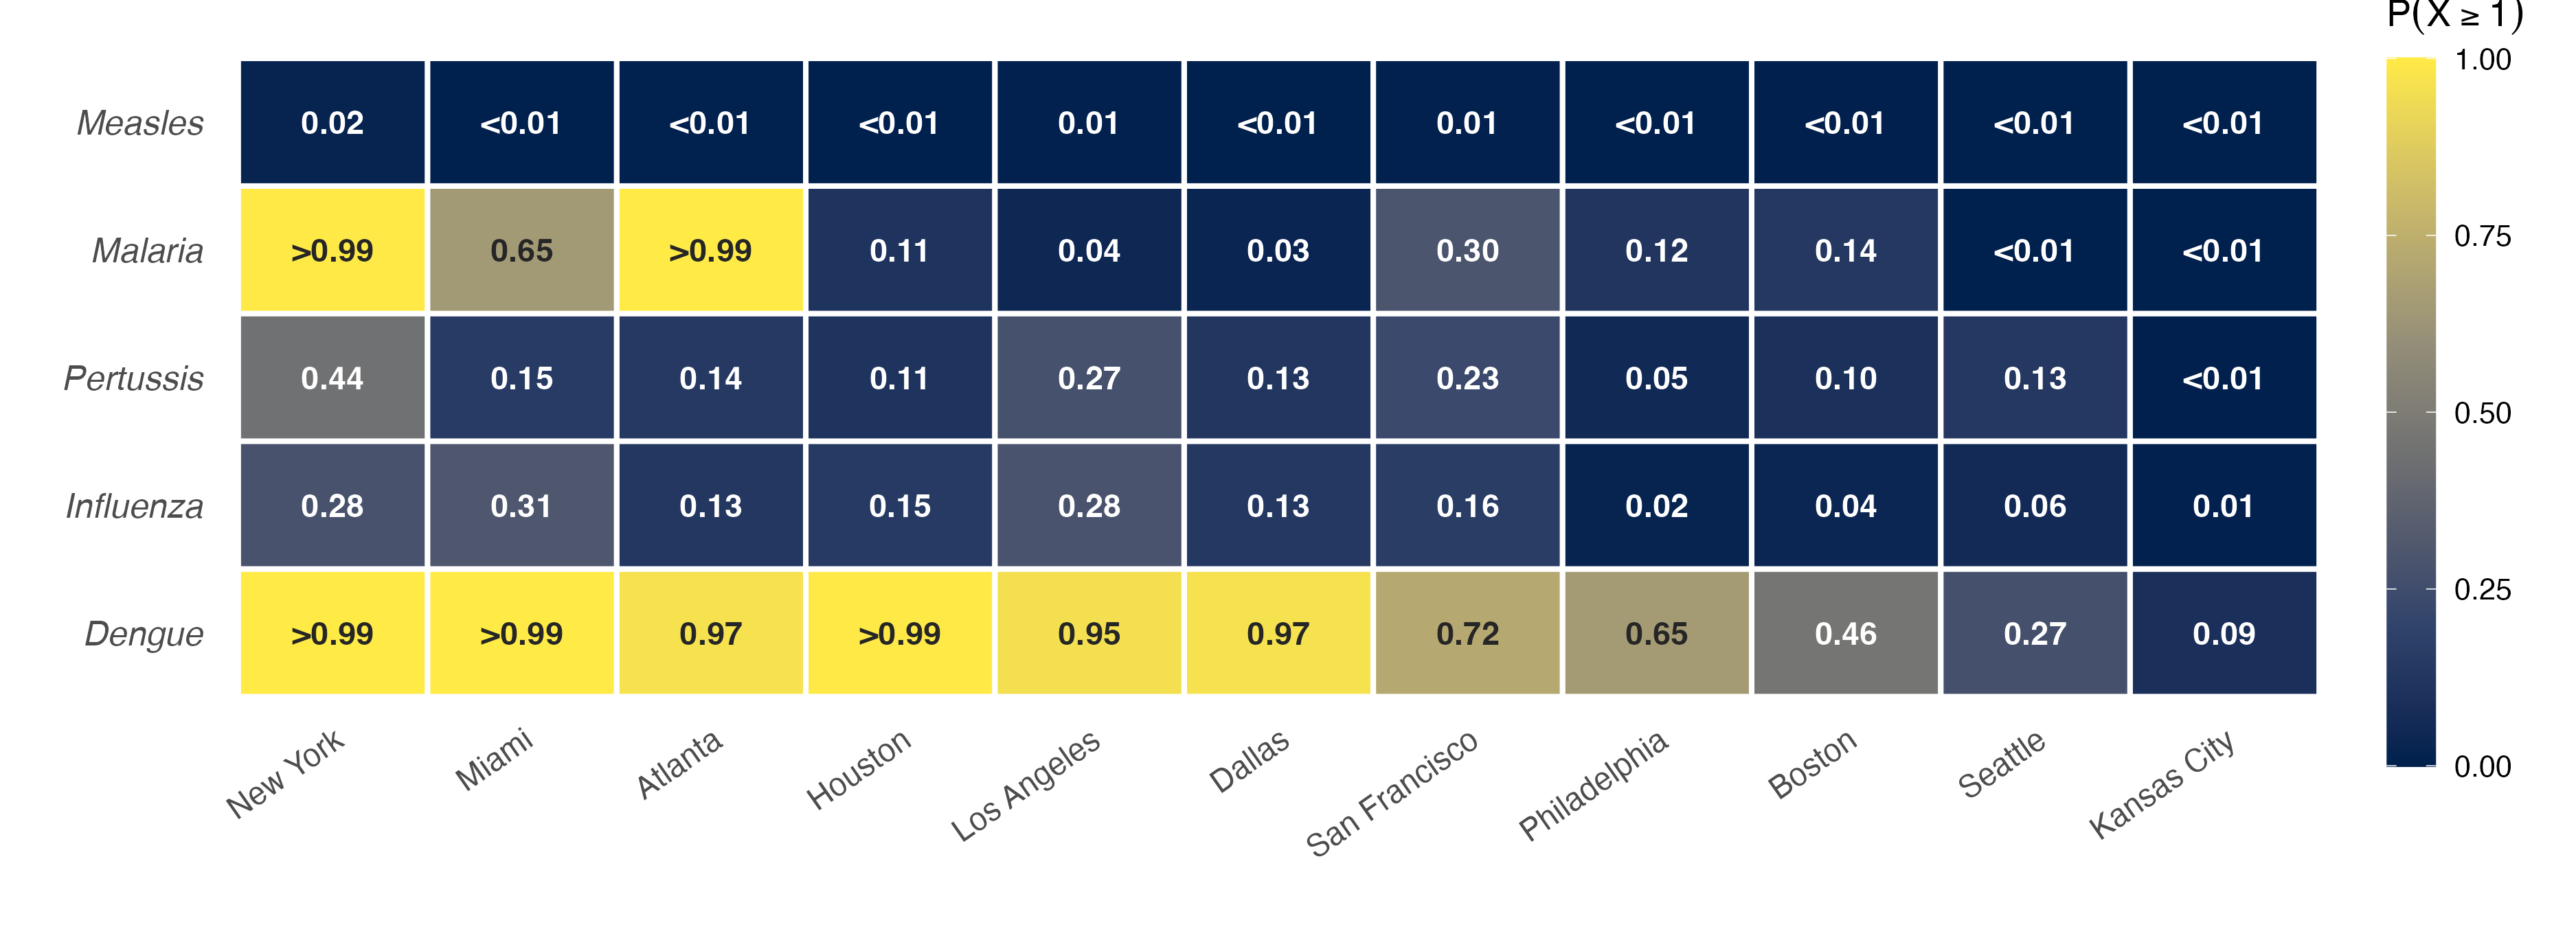
\includegraphics[width=\textwidth]{Figure1.png}
  \caption{\textbf{Importation probability for five infectious diseases at 11 US FIFA World Cup 2026 host cities.} Cells show $P(\geq 1)$, the probability of at least one imported case at each city in June 2026, under the schedule-driven model (M3) Monte Carlo median. Cities are ordered by total importation intensity. Values $<0.01$ and $>0.99$ are shown as such.}
  \label{fig:heatmap}
\end{figure}

\subsection{Expected importation intensity and parameter uncertainty}

Figure~\ref{fig:lambdaci} shows Monte Carlo median $\Lambda$ and 95\% uncertainty intervals for each disease and city. Dengue intensities are roughly 3-fold higher than malaria and nearly three orders of magnitude above measles. Interval asymmetry is disease-specific; for dengue, the upper interval bound is roughly twice the median while the lower bound is about one third of the median, indicating that the central estimate lies in the lower half of the plausible range. For pertussis, the upper CI is compressed toward the median, confirming that estimates are conservative upper bounds (the reference detection rate equals the upper literature limit).

\begin{figure}[htbp]
  \centering
  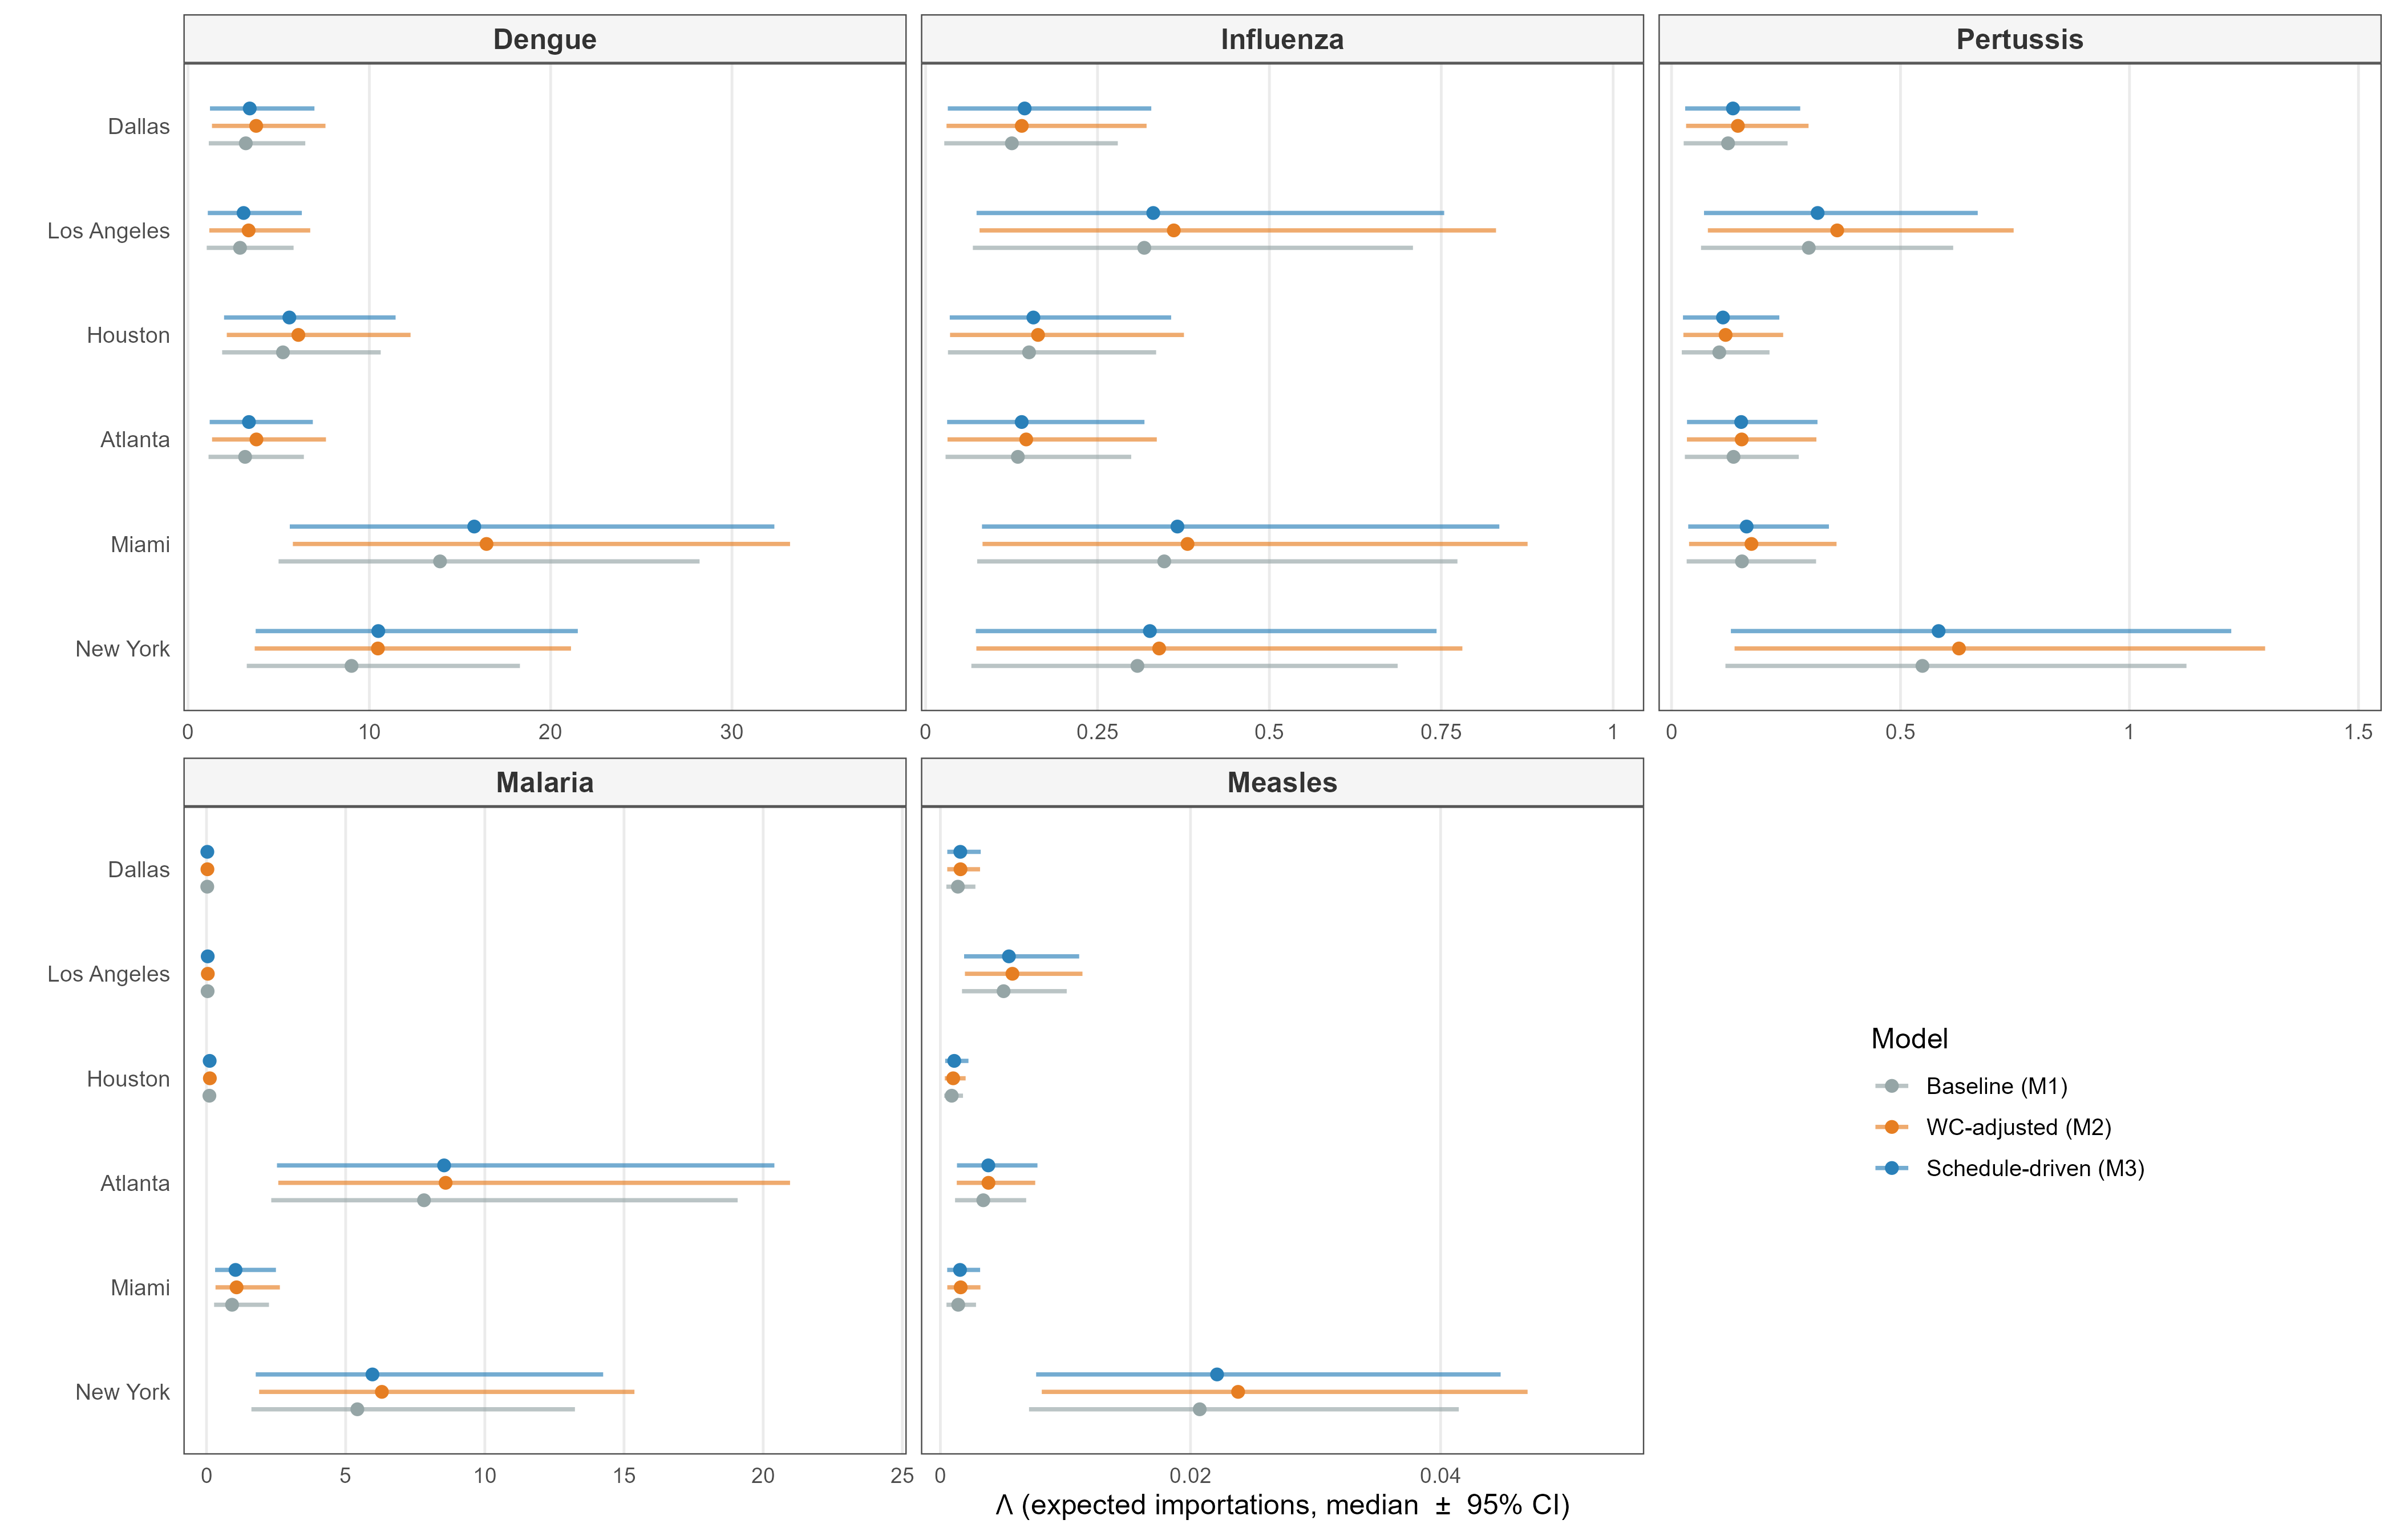
\includegraphics[width=\textwidth]{Figure2.png}
  \caption{\textbf{Three-model comparison of expected importation intensity ($\Lambda$) with 95\% Monte Carlo uncertainty intervals by disease across the six highest-risk US host cities.} Points are Monte Carlo medians; horizontal bars span the 2.5th--97.5th percentiles from 5,000 Uniform draws on $\rho_d$ and $p_d$. Interval asymmetry is examined in Supplementary Figure~S3. Each disease panel has an independent x-axis. Colors correspond to model:  M1 = Baseline (COR June 2024, no World Cup adjustment); M2 = WC-adjusted (2026 projections, T-100 routing for all travellers); M3 = Schedule-driven (World Cup fans routed by match schedule, background travellers by T-100).}
  \label{fig:lambdaci}
\end{figure}

\subsection{Effect of the World Cup travel surge across model tiers}
\label{sec:comparison}

The World Cup travel surge (M1 $\to$ M2) increased the 11-city dengue total by approximately 17\% (39.7 to 46.6; Figure~\ref{fig:lambdaci}). The schedule-driven model (M3: 45.0) fell slightly below the WC-adjusted model (M2: 46.6) because the fan increment for teams playing in Canada and Mexico was redirected to non-US venues, reducing US city totals. M2 allocates all World Cup growth to US cities via T-100 routing and cannot make this distinction, so M3 gives a more accurate estimate of the US-specific burden. Comparable patterns held for malaria (M1: 14.7, M2: 16.6, M3: 16.4) and the other diseases.

% \begin{figure}[htbp]
%   \centering
%   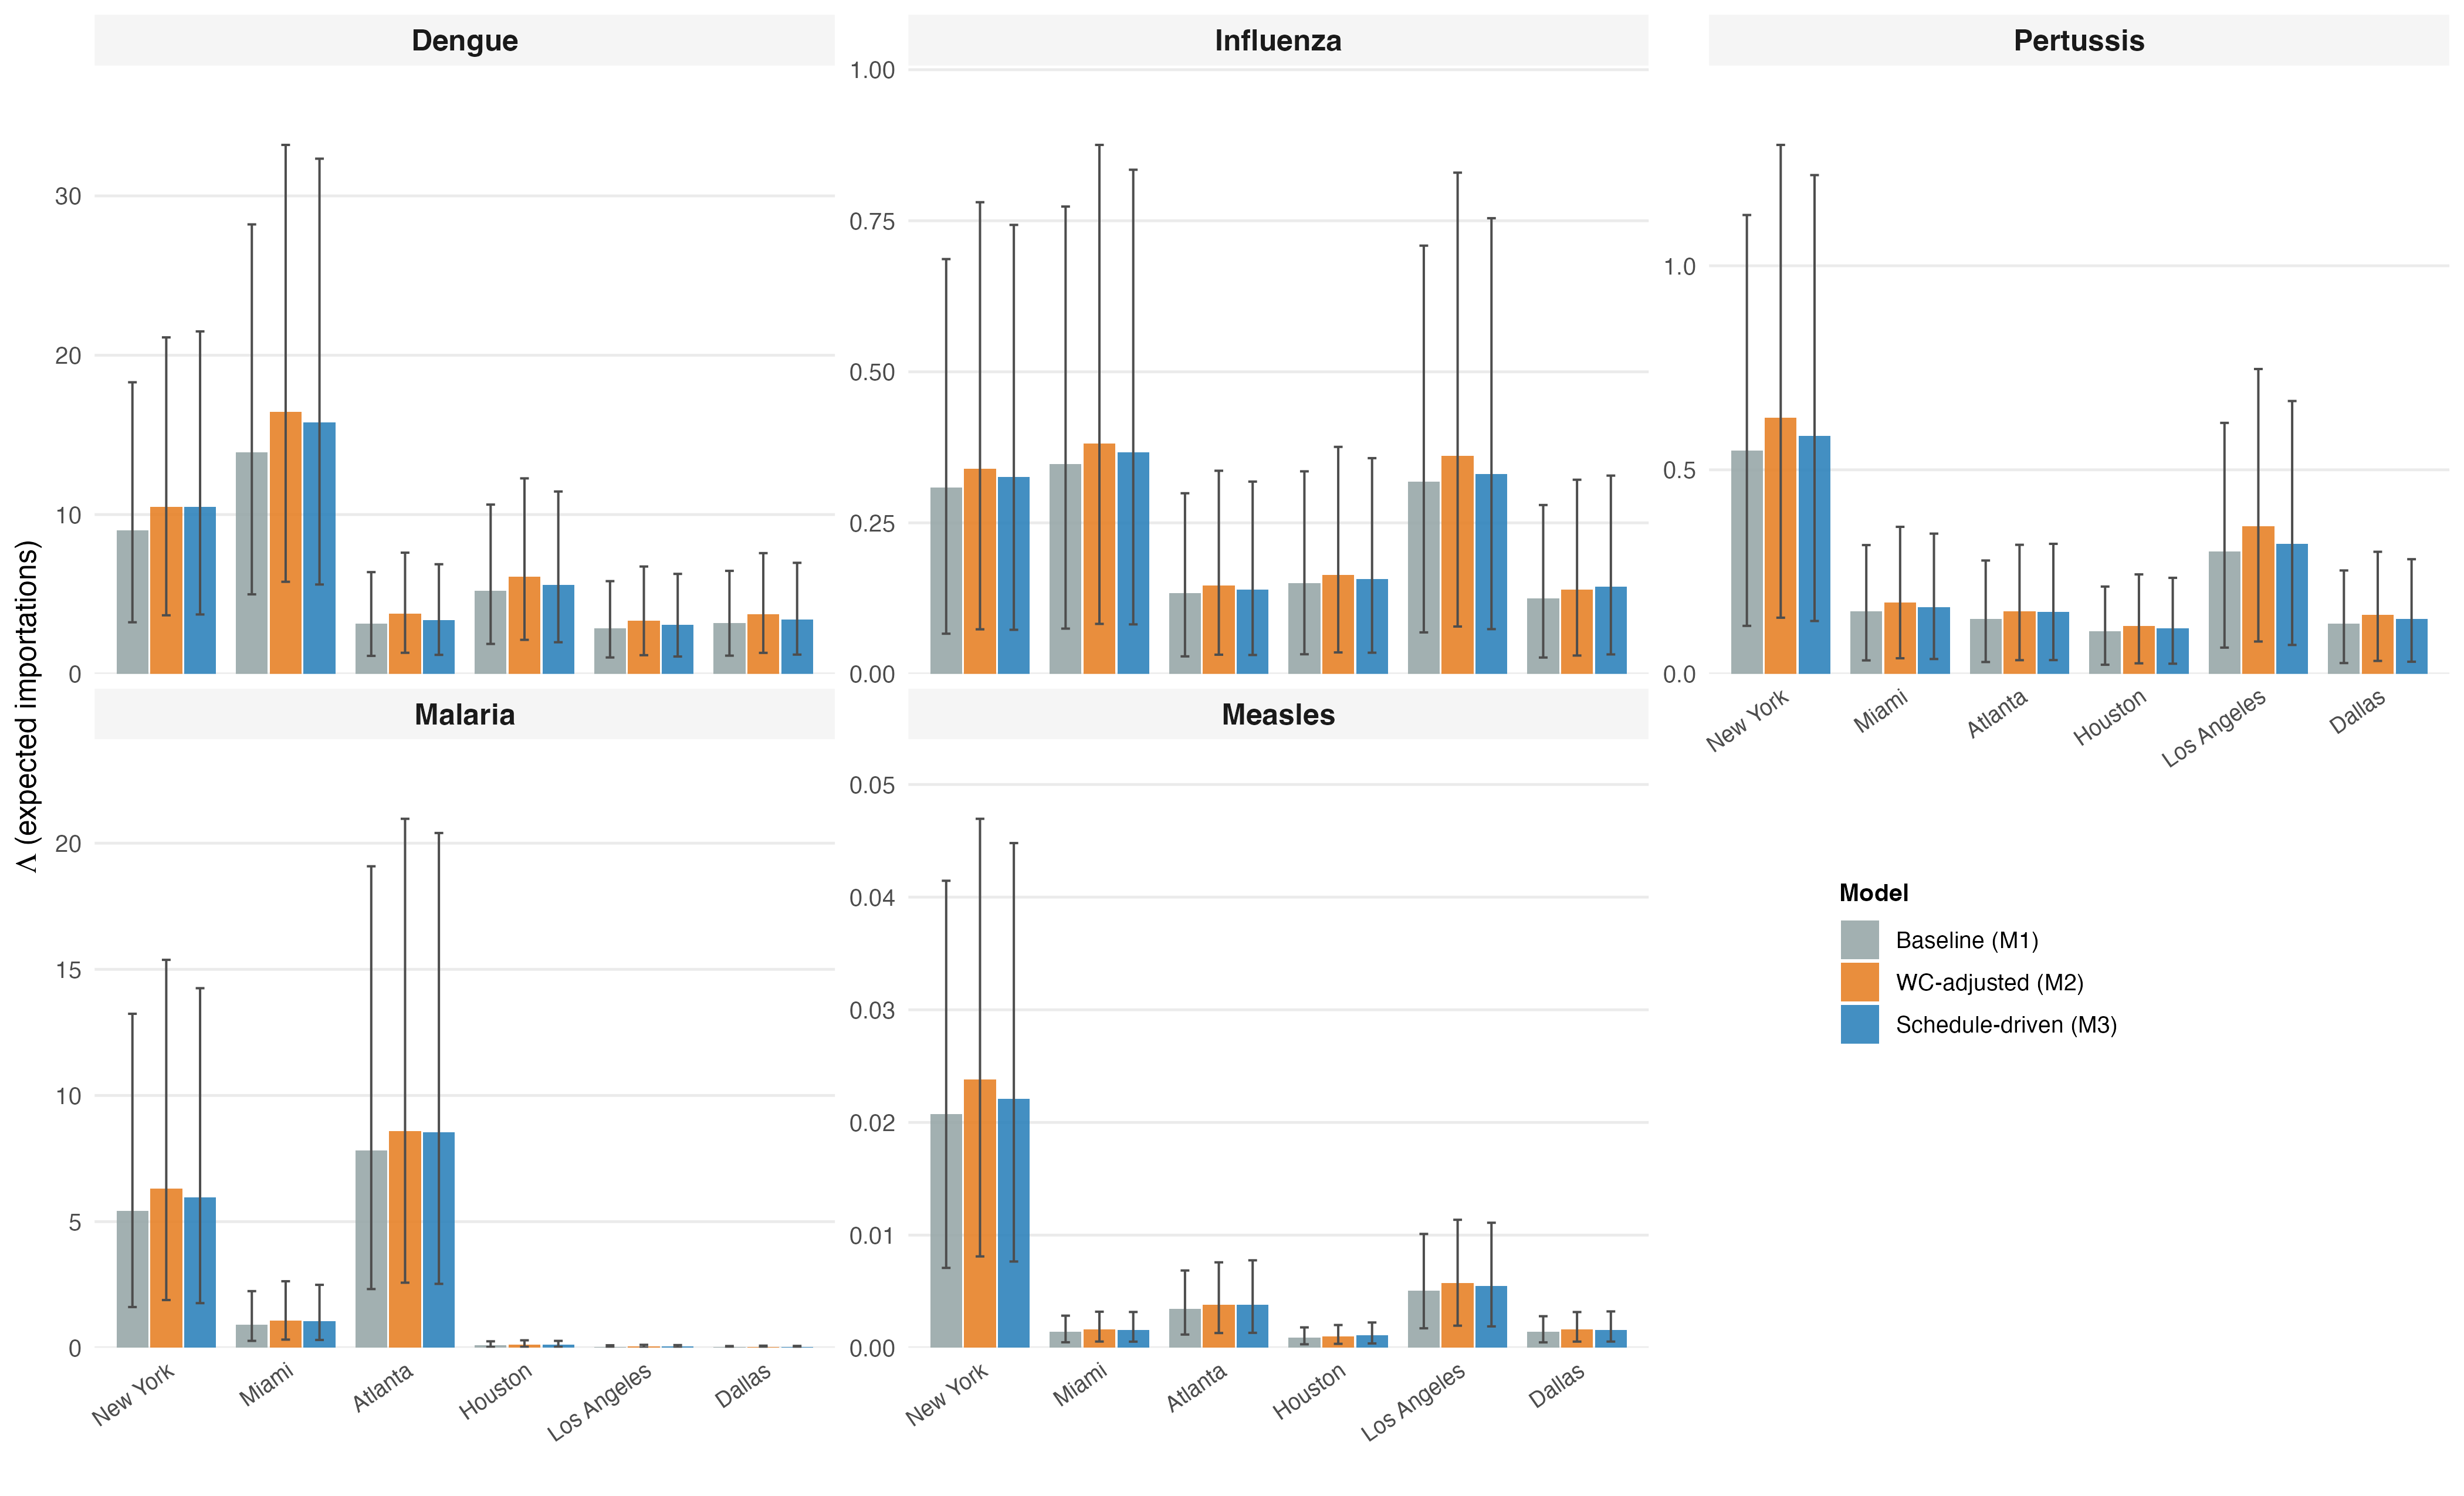
\includegraphics[width=\textwidth]{fig3_model_comparison_IJID.png}
%   \caption{\textbf{Three-model comparison of expected importation intensity for the six highest-risk US host cities.} Bars show Monte Carlo median $\Lambda$; error bars show 95\% uncertainty intervals. M1 = Baseline (COR June 2024, no World Cup adjustment); M2 = WC-adjusted (2026 projections, T-100 routing for all travellers); M3 = Schedule-driven (World Cup fans routed by match schedule, background travellers by T-100). Panels use free y-axes; note differences in scale across diseases.}
%   \label{fig:lambdaci}
% \end{figure}

Figure~\ref{fig:excess} decomposes the 11-city total into baseline travel (M1) and the World Cup-specific increment (M3 $-$ M1) for each disease. Baseline travel accounts for 86--93\% of total expected importations across all diseases; the World Cup adds only 7--14\%. Most of the risk is thus present without the tournament, and surveillance confined to the World Cup window will miss most of it.

\begin{figure}[htbp]
  \centering
  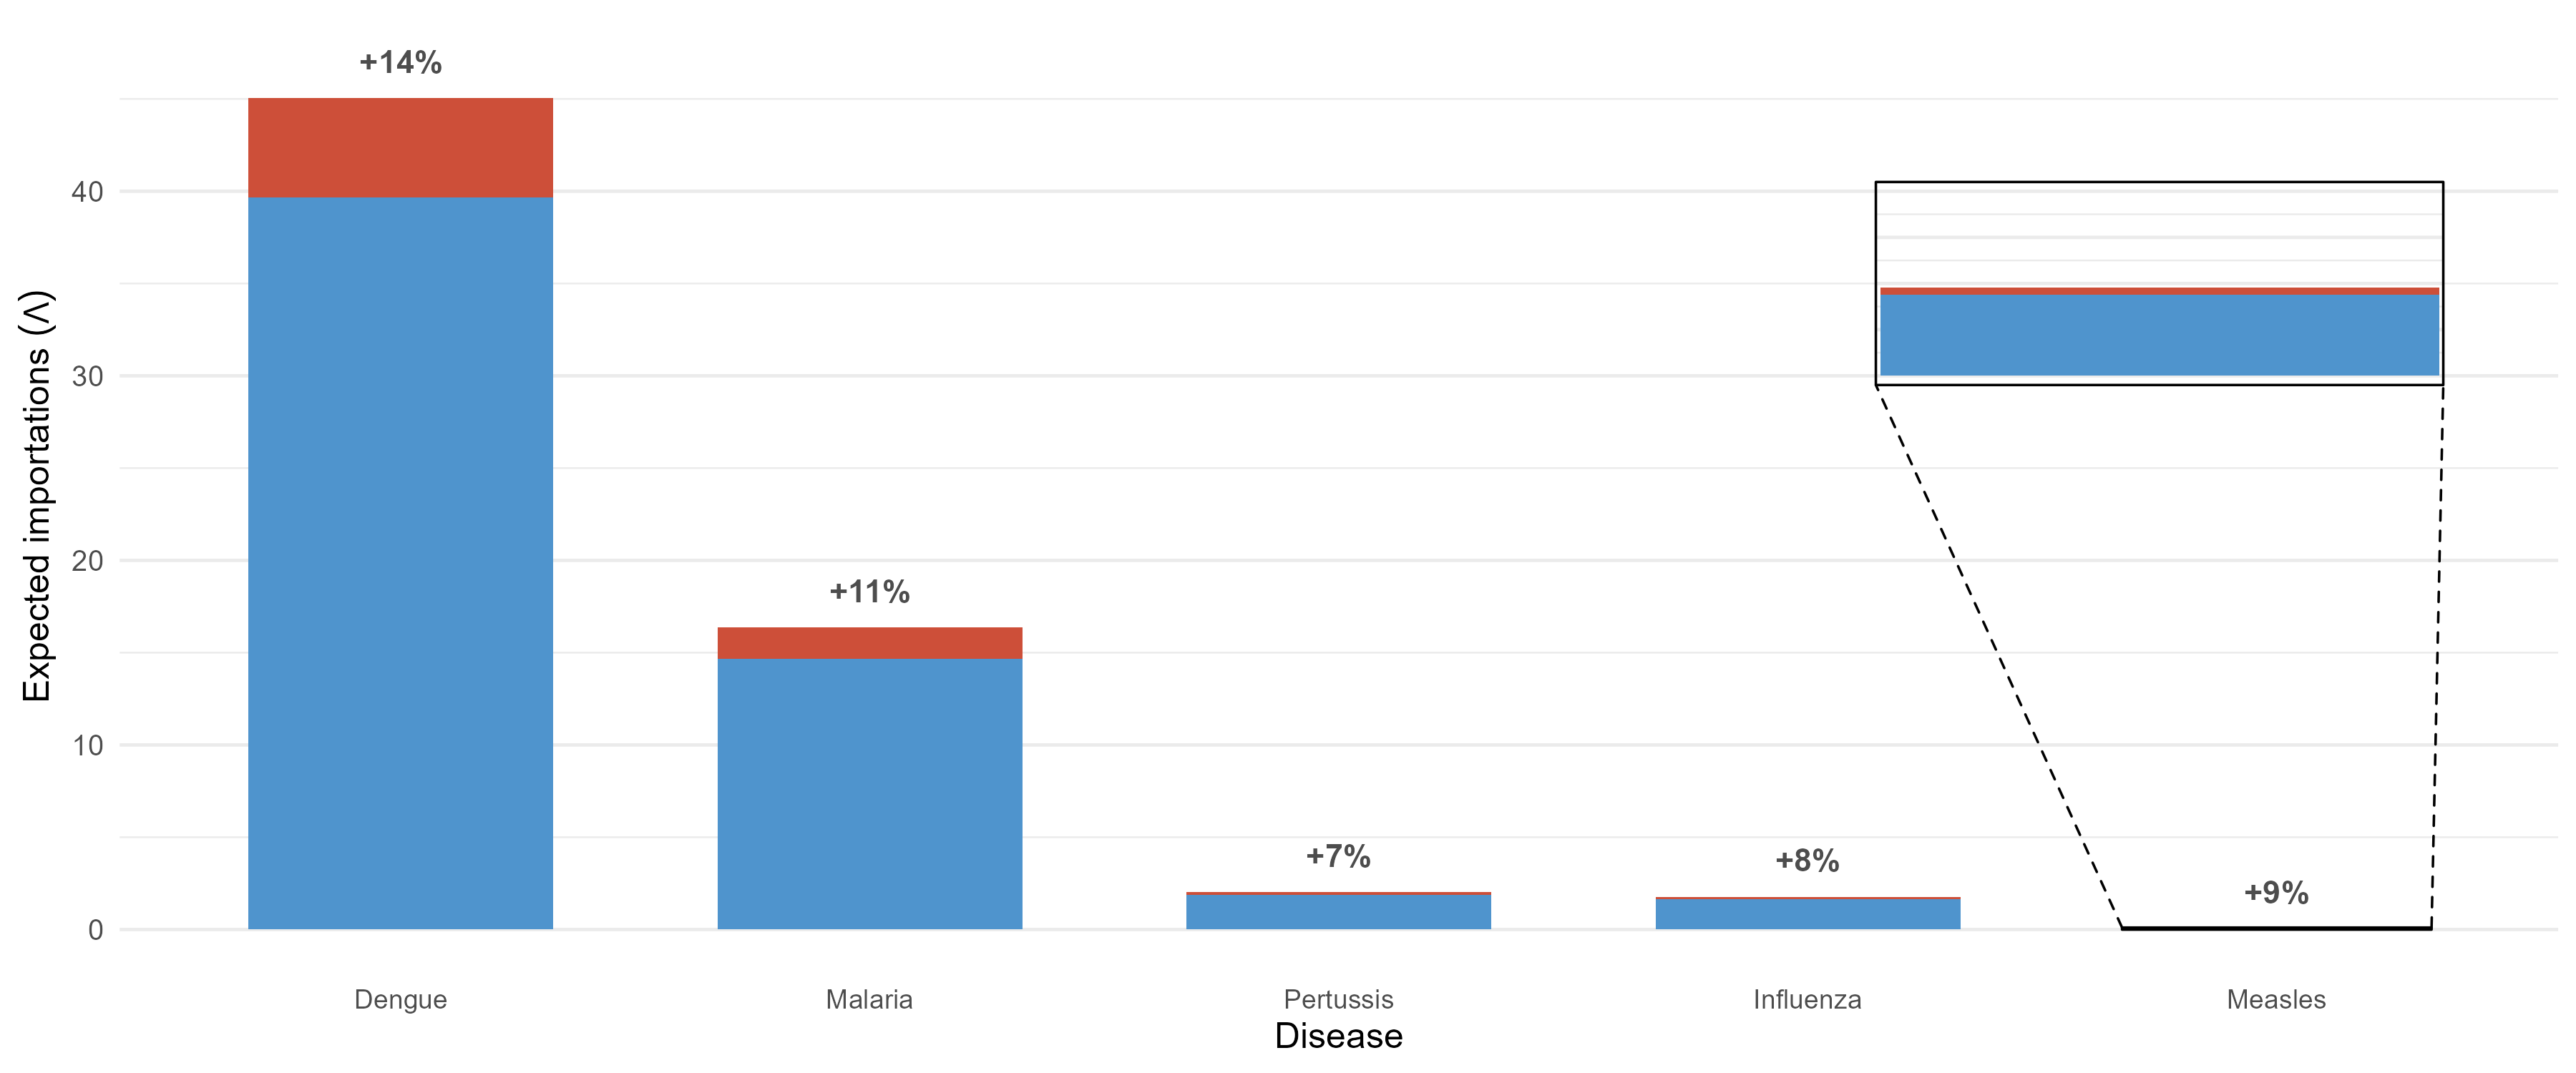
\includegraphics[width=\textwidth]{Figure3.png}
  \caption{\textbf{World Cup travel increment above baseline importation by disease.} Each bar shows the 11-city Monte Carlo median $\Lambda$ split into baseline travel (M1, blue) and the schedule-driven WC increment (M3 $-$ M1, red). Percentage labels indicate the WC increment as a share of the M1 baseline. The inset shows a zoomed view of the estimates for measles, which are otherwise not visible on the same scale as the other diseases. Baseline travel dominates across all five diseases, contributing 86--93\% of total expected importations.}
  \label{fig:excess}
\end{figure}

\subsection{Source-country contributions}

Brazil and Mexico were the dominant dengue contributors across New York, Miami, and Houston (Figure~\ref{fig:countries}). Nigeria and Ghana drove malaria risk at Atlanta and New York. For dengue at World Cup fan countries, contributions were split between a fan-specific stream (concentrated at match venues) and a background stream (distributed by routine T-100 routing). This confirms that the surge amplification is real but built on pre-existing high baseline travel from endemic source countries. Supplementary Figure~S6 ranks the same top-10 source countries by diaspora-weighted importation intensity ($\Omega^A$) rather than raw $\lambda$; countries with large co-national communities concentrated in their primary destination cities rank higher in $\Omega^A$ than in $\lambda$, revealing an additional layer of community-level exposure not visible from travel volumes alone.

\begin{figure}[htbp]
  \centering
  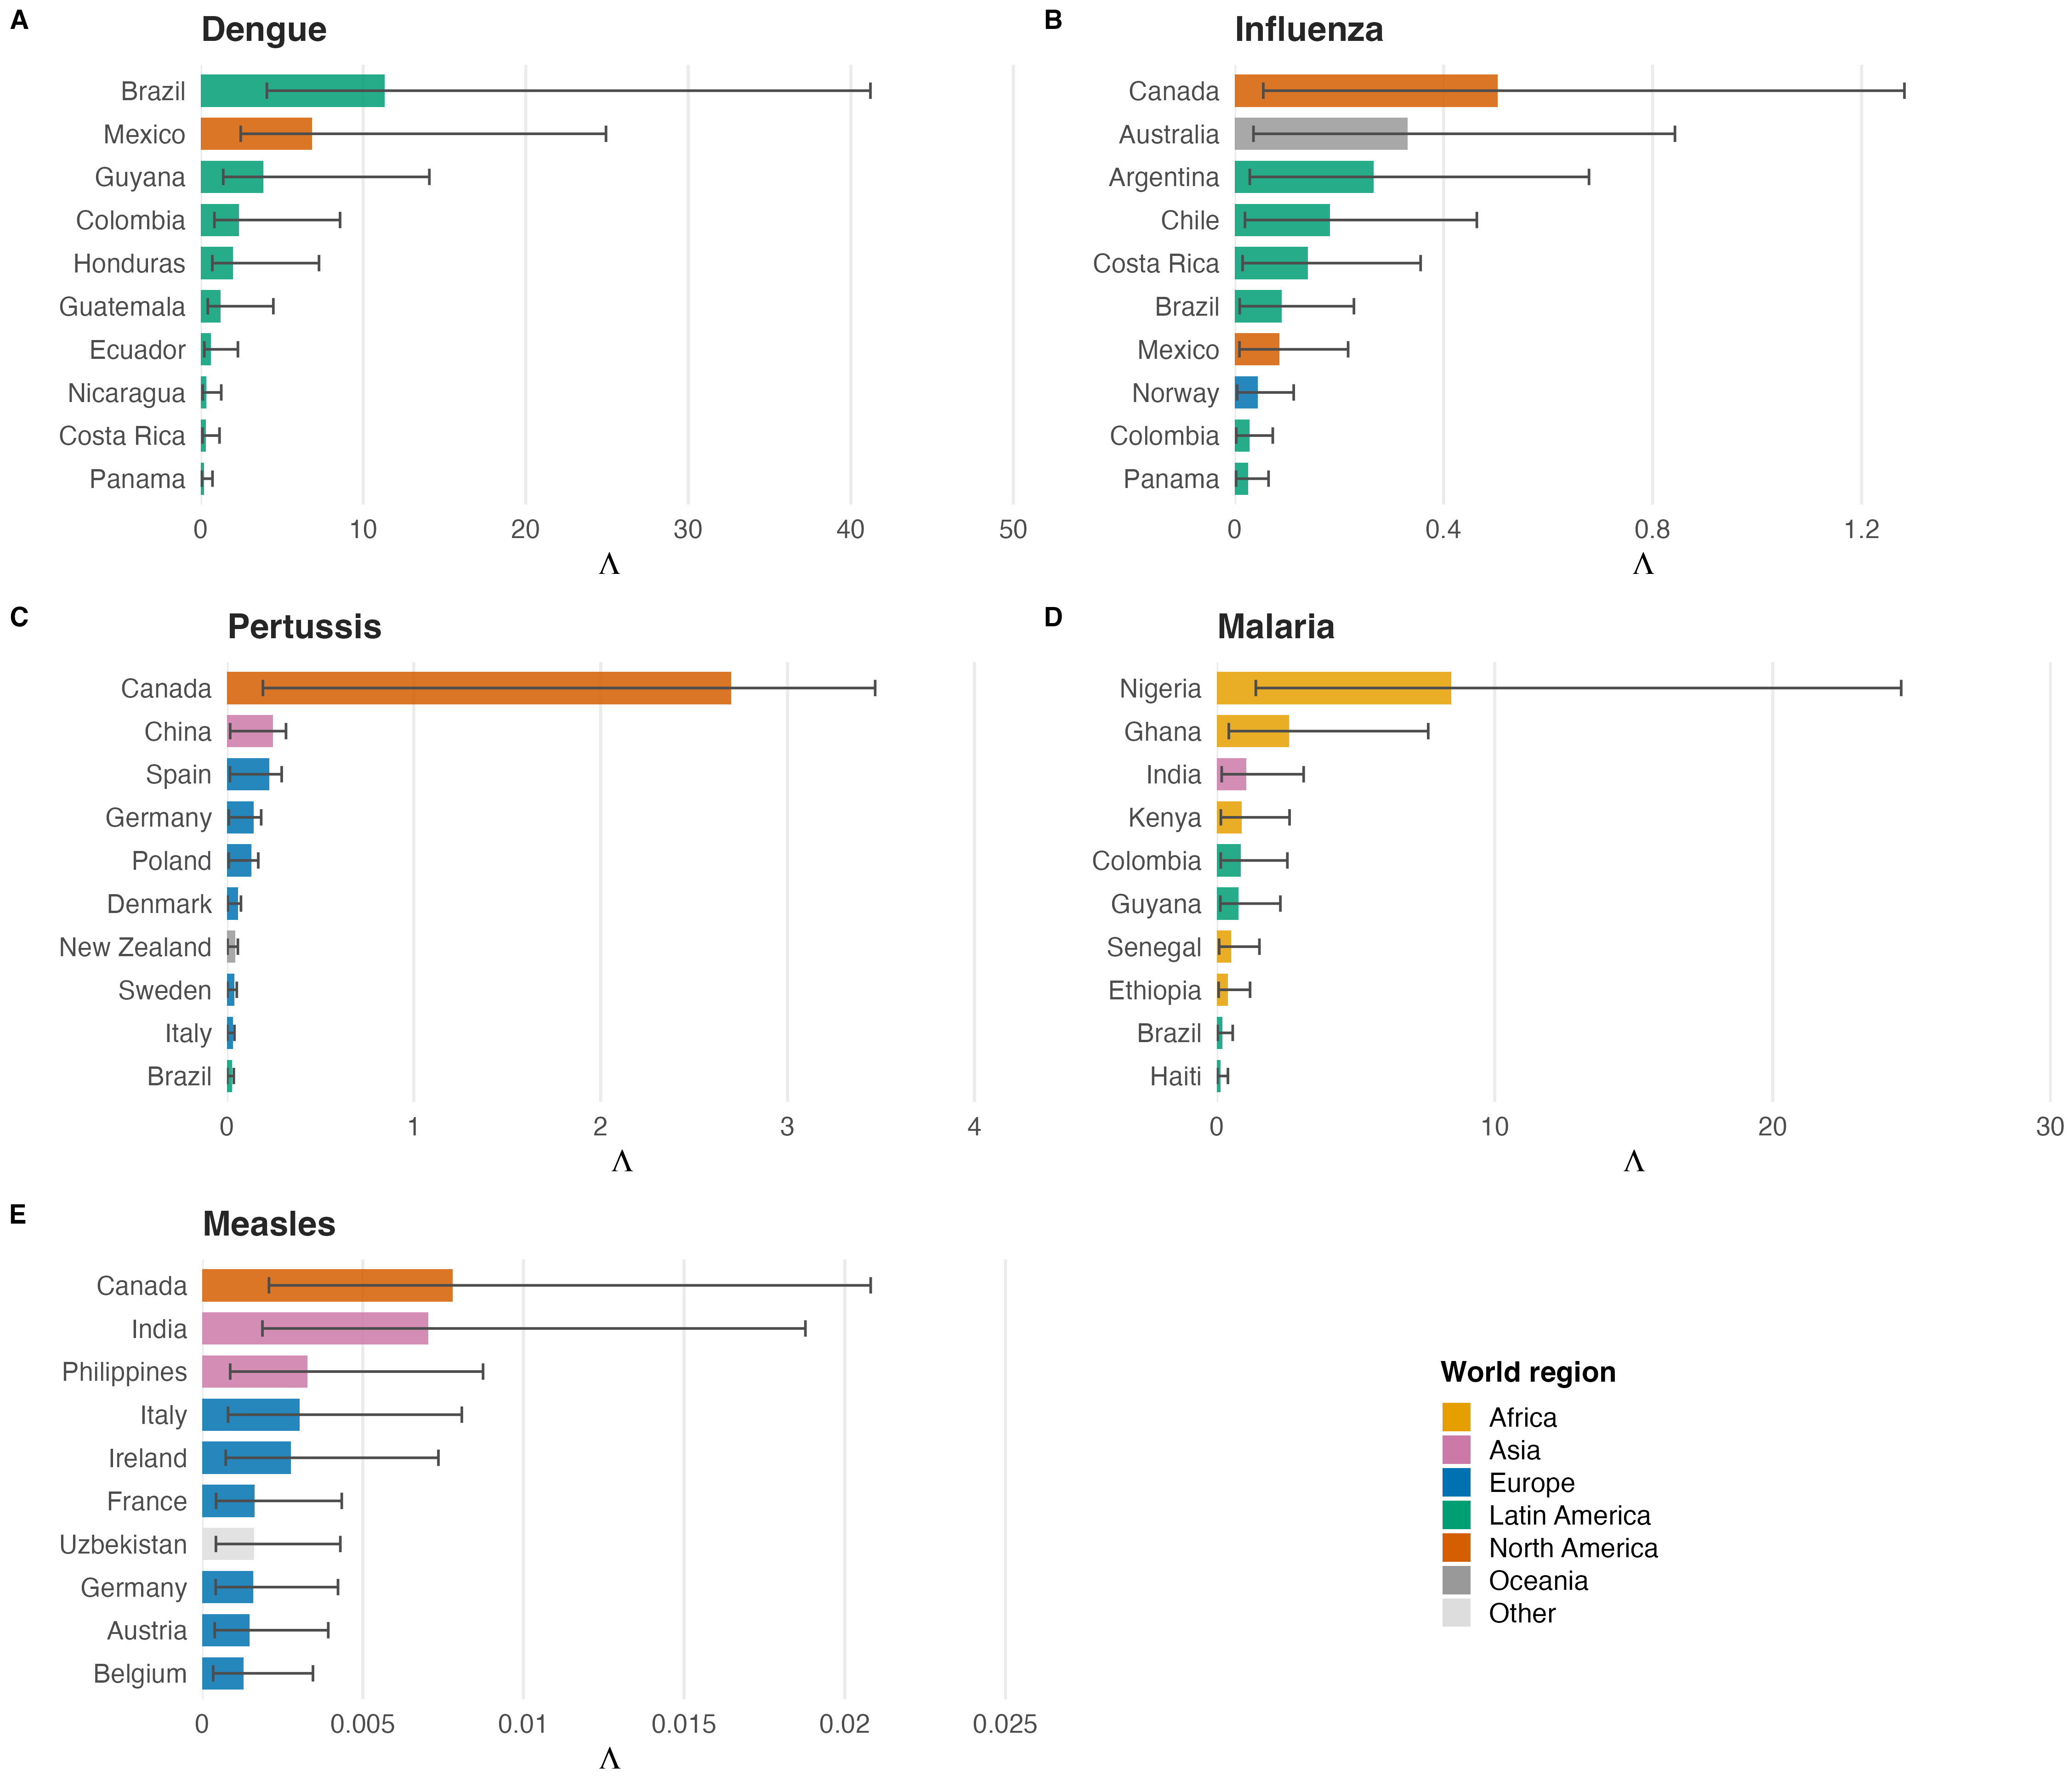
\includegraphics[width=\textwidth]{Figure4.png}
  \caption{\textbf{Top 10 source-country contributors to expected importation intensity by disease, under the schedule-driven model (M3).} Bars show expected importations $\lambda_{c,\cdot,d}$ summed across all 11 US venue cities; error bars show 95\% Monte Carlo uncertainty intervals. Colors denote world region (Canada and Mexico grouped as North America). Panels: (A)~dengue, (B)~influenza, (C)~pertussis, (D)~malaria, (E)~measles.}
  \label{fig:countries}
\end{figure}

\subsection{Diaspora network seeding risk}

Figure~\ref{fig:diaspora} summarizes both diaspora risk mechanisms for dengue and malaria, the two diseases with meaningful diaspora signal. Panel A shows $P^A(\geq 1)_{v,d}$, the probability that at least one imported case enters a co-national diaspora social network at each host city. For dengue, the diaspora signal was highest at Dallas, Houston, and Los Angeles ($P^A(\geq 1) = 0.43$, $0.39$, and $0.35$), driven by the large Mexican diaspora in these cities ($\kappa = 0.39$, $0.34$, and $0.34$); Miami ($P^A(\geq 1) = 0.26$) was the exception, driven by its Colombian and Brazilian communities ($\kappa = 0.076$ and $0.025$). Although dengue importation is very likely at the city level in these metropolitan areas ($P(\geq 1) > 0.95$; Figure~\ref{fig:heatmap}), the probability that an imported case enters a co-national diaspora network is much lower ($P^A(\geq 1) \le 0.43$), indicating that most imported dengue risk disperses into the general urban population rather than concentrating within a single co-national community. For malaria, Atlanta showed the highest $P^A(\geq 1)$ ($0.23$), reflecting the high malaria importation intensity routed through Hartsfield-Jackson airport channeled into the city's Nigerian diaspora ($\kappa = 0.031$).
 
Panel B shows the Mechanism B secondary seeding index ($\Omega^B$): the importation intensity at a match venue weighted by the diaspora concentration of the home metropolitan area to which fans return, evaluated across the 11 host cities and 15 major non-host metropolitan areas. For dengue, the seven highest-ranked hubs were all non-host cities with large Mexican diaspora populations — San Antonio ($\Omega^B = 4.1$), Phoenix ($3.4$), San Diego, Denver, Chicago, Austin, and Las Vegas — each ranking above the leading host-city hub (Dallas, $2.3$). For malaria, secondary seeding was more evenly divided between host cities (Houston, Dallas, Philadelphia, and Boston) and non-host cities (Washington, DC; Minneapolis; Austin; Charlotte; Detroit; and Chicago), reflecting their Nigerian and Indian diaspora communities (Supplementary Figure ~S8). Results for all five diseases are provided in Supplementary Figure~S5. The full Mechanism A diaspora probability ($P^A(\geq 1)$) across all five diseases and 11 host cities is provided in Supplementary Figure~S7.

\begin{figure}[htbp]
  \centering
  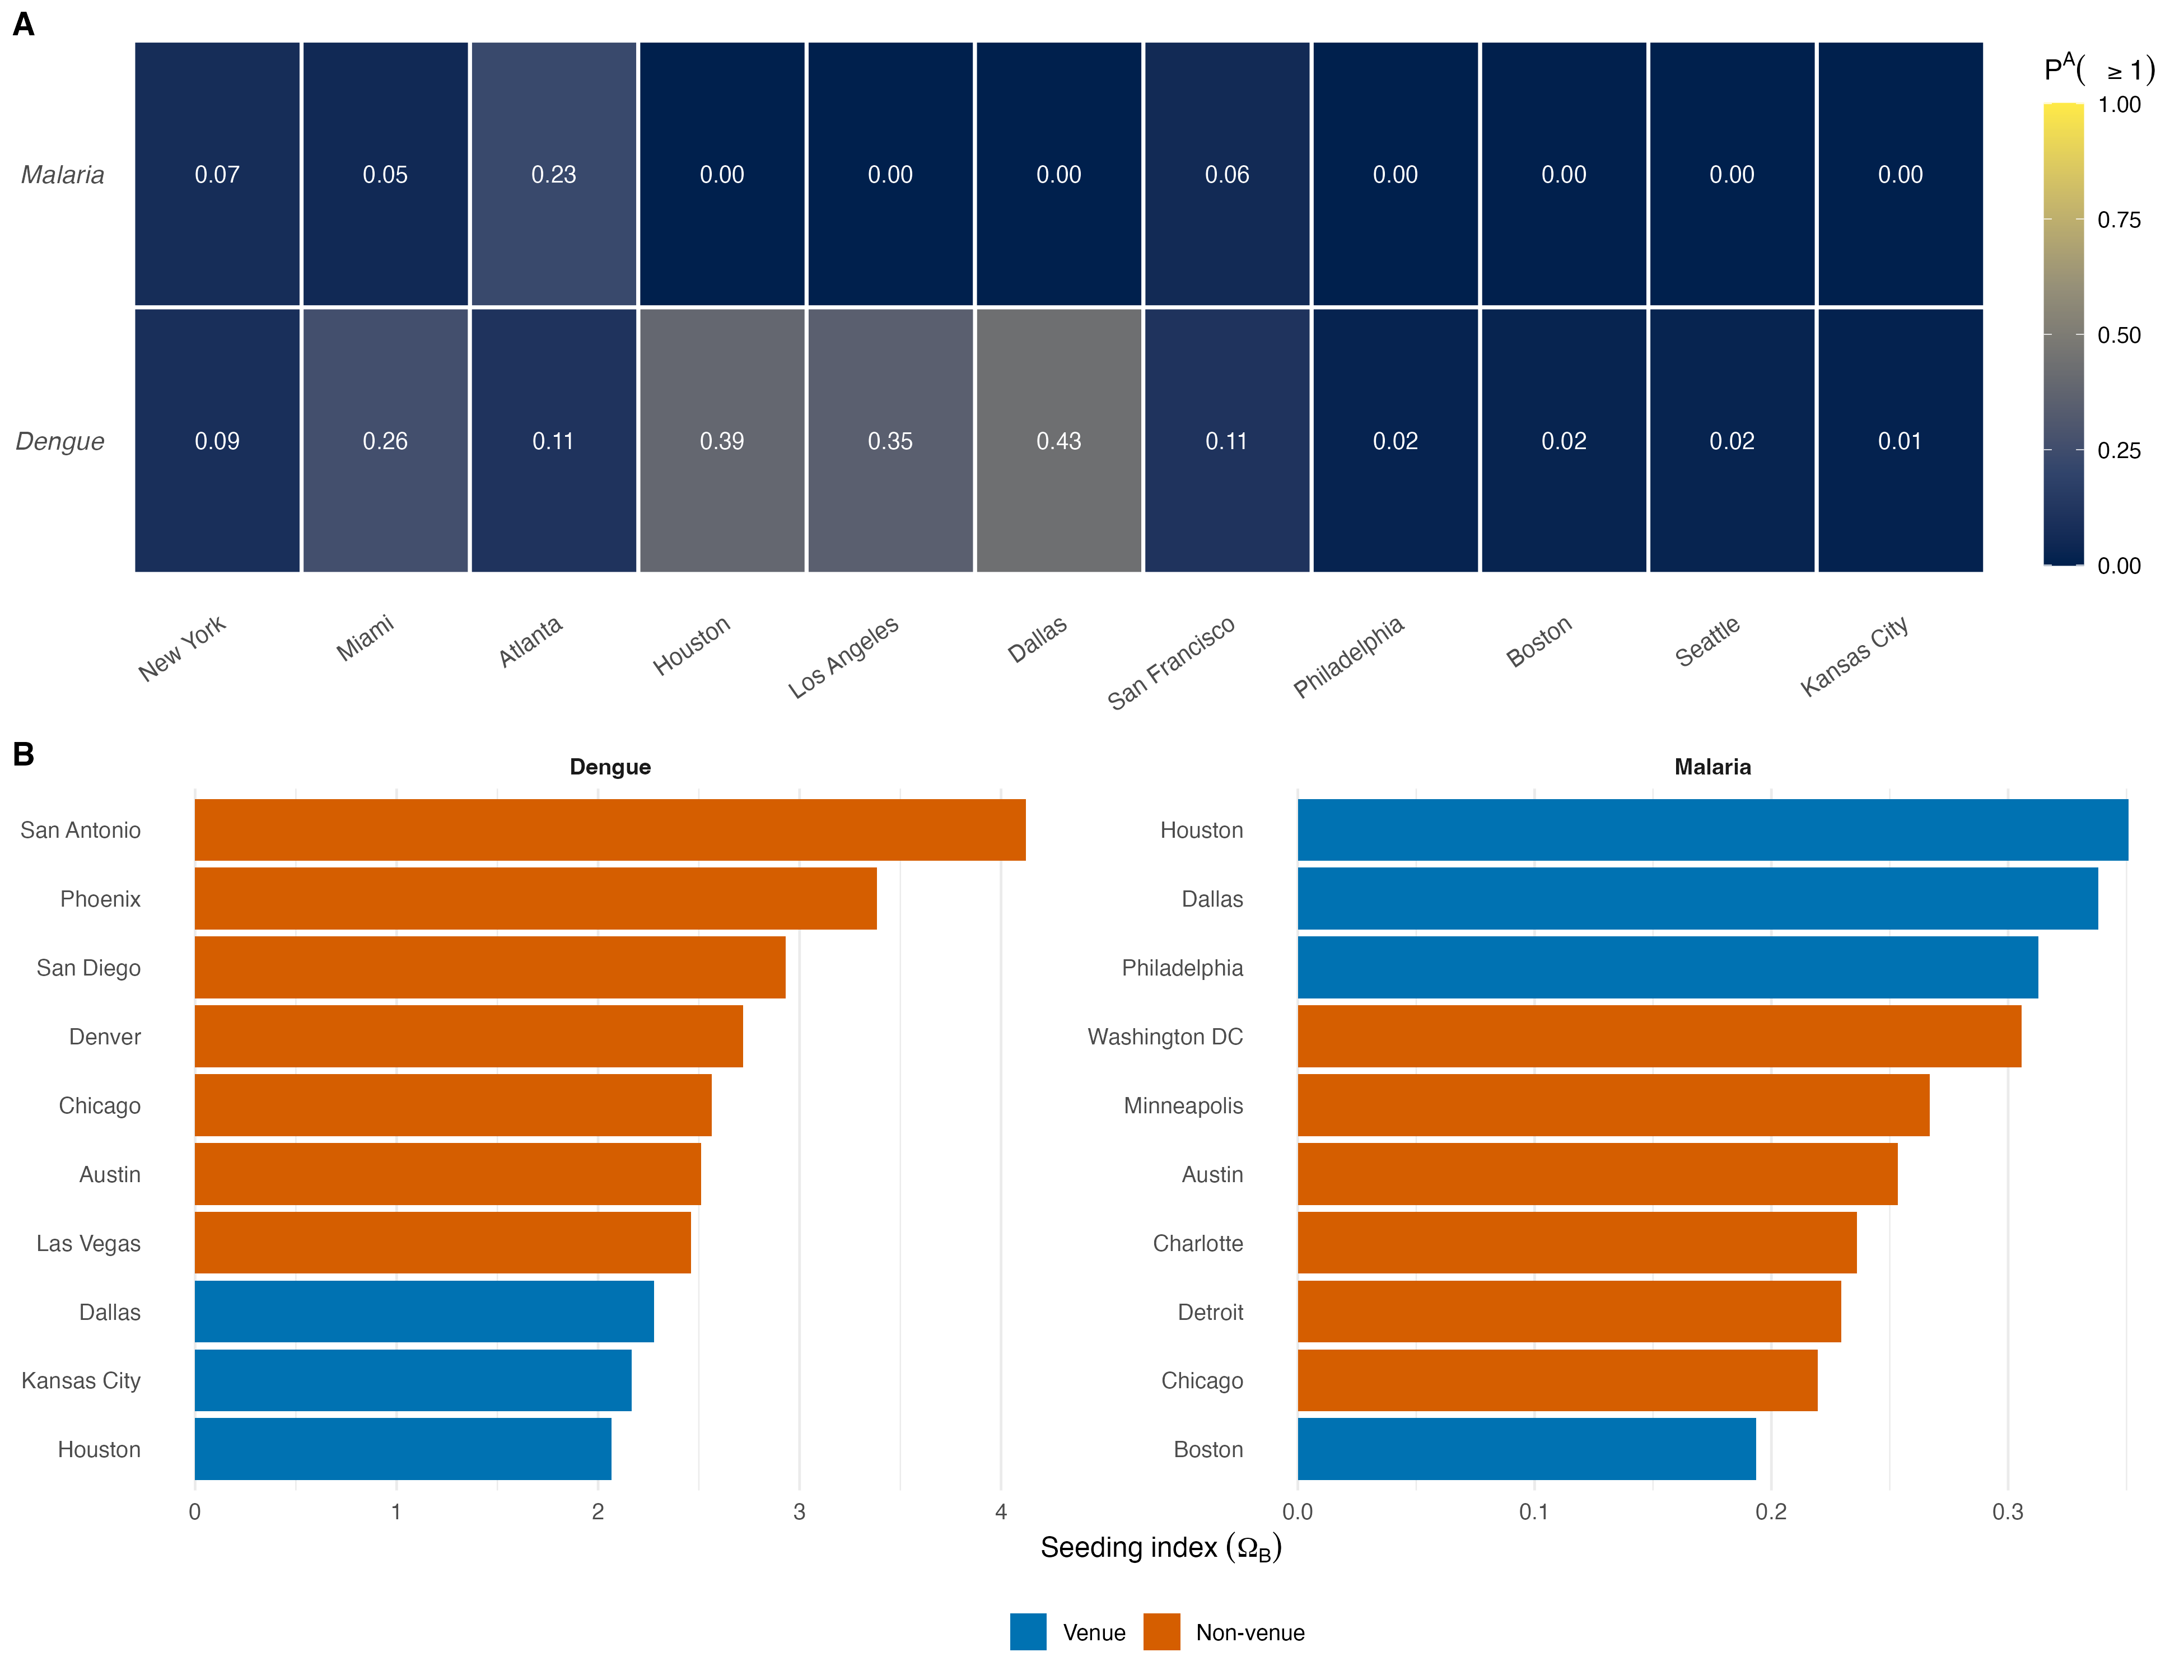
\includegraphics[width=\textwidth]{Figure5.png}
  \caption{\textbf{Diaspora network seeding risk for dengue and malaria.}
    \textbf{Panel A (Mechanism A):} probability that at least one imported case enters a co-national diaspora network at each host city, $P^A(\geq 1)_{v,d}$. \textbf{Panel B (Mechanism B):} secondary seeding index $\Omega^B$ for the top 10 hub metropolitan areas per disease, colored by whether the hub is a World Cup host city or a non-host city. Hubs are the home cities to which fans return after attending matches.}
  \label{fig:diaspora}
\end{figure}

% =============================================================
\section{Discussion}
% =============================================================

Dengue presents the highest importation risk across the 11 host cities. Miami, New York, and Houston each reach $P(\geq 1) > 0.99$ under M3, driven by high June dengue burden in WC-qualified Latin American nations, large bilateral travel volumes, and a relatively wide infectious-but-travel-capable window ($p_d = 0.30$--$0.70$). Dallas and Atlanta reach $P(\geq 1) > 0.95$; the remaining venues fall substantially below that threshold. The 11-city dengue total carries a right-skewed uncertainty distribution (median 45.0, 95\% CI 16.0--92.3), due to the reference under-reporting correction ($\rho_d = 0.10$) sits near the lower end of the literature range (0.06--0.26), the upper bound of 92.3 is therefore a plausible outcome, and the median should be read as a conservative estimate.

In 2024, 3,798 travel-associated dengue cases were reported in the US --- a 359\% increase over the historical average \citep{Kiplagat2026dengue} --- consistent with the high modeled baseline. Although 2025 incidence moderated, routine bilateral travel from endemic Latin American nations sustains this pre-existing risk; the World Cup surge adds a further 7--14\% above baseline. M3 differs from M2 because fan travel for teams playing in Canada or Mexico is routed to those venues rather than distributed across US cities via T-100 fractions. For dengue, this reduces the 11-city M2 total (46.6) to the M3 estimate (45.0), a 3\% downward adjustment that varies by venue depending on the match schedule. Preparedness resources calibrated to M3 are therefore directed to the cities where fan flows actually land.

The most policy-relevant finding is that baseline travel accounts for 86--93\% of total expected importations across all five diseases (Figure~\ref{fig:excess}). The World Cup adds 7--14\% above a risk that exists every June, tournament or not. Year-round monitoring of international travelers arriving at US airports from endemic regions is therefore indispensable; targeted tournament-period surveillance is a complement, not a substitute. The marginal contribution of the WC travel surge is real but modest relative to the structural baseline, and any risk assessment that  excludes a pre-tournament counterfactual will overstate it.

The diaspora extension asks whether an imported case enters a concentrated co-national social network or disperses into the general population, a distinction absent from standard importation models. This distinction is operationally important because co-national networks have higher contact rates for disease transmission, may face language and access barriers to healthcare, and are often the focus of World Cup watch-party gatherings that could amplify early transmission chains. The $P^A(\geq 1)$ metric provides a directly actionable quantity for targeted community health outreach that complements city-level $P(\geq 1)$ monitoring.

Our analysis has several limitations. First, Poisson assumes independence and equates mean with variance; correlated arrivals from coordinated group travel by fans from the same country introduce overdispersion, so variance is understated and uncertainty bounds are narrower than the true sampling distribution warrants. Second, $\rho_d$ corrects for under-reporting in source-country surveillance but does not model US detection rates; our $\Lambda$ estimates represent true infected arrivals, not detected US cases, so comparisons with CDC surveillance tallies require additional adjustment. Third, $C_{c,d}/P_c$ uses total-population incidence without age stratification, which introduces directional biases that vary by disease; malaria risk from high-endemic sub-Saharan African settings is likely overestimated because pediatric cases dominate reported burden while adult travelers typically carry partial acquired immunity through repeated prior exposure, whereas for pertussis the bias is smaller because waning vaccine-induced immunity has progressively shifted burden toward the young-adult traveler demographic. Fourth, diaspora concentration $\kappa_{c,v}$ is derived from ACS 2019--2023 data spanning the COVID-19 pandemic, which altered immigration patterns; values may not perfectly reflect the June 2026 population distribution. Fifth, the analysis covers only the 11 US host cities; Canadian and Mexican venues, which receive meaningful World Cup fan flows, are outside the primary scope. Sixth, the near-zero measles estimate reflects the model's scope --- it estimates independent seeding events, not outbreak chains; US measles case counts typically arise from a small number of imports followed by local transmission in undervaccinated communities, a process not captured by the Poisson framework. Seventh, the World Cup growth factors $\phi_c$ are derived from NTTO point projections and treated as deterministic; uncertainty in fan-travel forecasts is not propagated into the reported intervals, so the true uncertainty bounds are likely wider than reported for M2 and M3 estimates. Finally, because $p_d$ enters multiplicatively it is a key driver of uncertainty; a one-parameter sensitivity analysis (Table~S1) confirms that malaria and measles estimates are most sensitive to this parameter (fold-change up to 5.0$\times$ across the literature range), while pertussis is least sensitive (1.8$\times$); absolute importation counts at each $p_d$ level are provided in the analysis code repository.

% =============================================================
\section{Conclusions}
% =============================================================

Dengue importation probability exceeds 0.99 in Miami, New York, and Houston, and exceeds 0.95 in Dallas and Atlanta; malaria is the dominant threat in Atlanta and New York, where $P(\geq 1)$ also exceeds 0.99. Baseline travel accounts for 86--93\% of total expected importations across all diseases, confirming that the dominant risk exists year-round independently of the tournament; the World Cup travel surge contributes a real but modest 7--14\% increment above that pre-existing burden. A two-tier surveillance strategy is warranted, combining increased city-level monitoring for dengue and malaria with targeted community outreach within co-national diaspora networks at Dallas, Houston, Los Angeles, and Miami, where $P^A(\geq 1)$ reaches 0.43, 0.39, 0.35, and 0.26, respectively. The schedule-driven Poisson framework is directly reusable for future mega-events by substituting updated travel volumes and disease incidence data, and its reliance on publicly available inputs makes it a practical first-pass tool for public health agencies planning risk assessments for any large international gathering.

% =============================================================
% DECLARATIONS
% =============================================================
\section*{Conflict of interest}
The author declares no conflict of interest.

\section*{Funding}
This research received no specific grant from any funding agency in the public, commercial, or not-for-profit sectors. J.L.H-D.\ acknowledges the support of the Department of Mathematics at Tarleton State University.   

\section*{Data availability}
All disease data are publicly available from WHO repositories cited
below. BTS T-100 and COR/I-94 travel data are available from the
Bureau of Transportation Statistics and US Customs and Border
Protection respectively. Diaspora data were obtained from the
US Census Bureau ACS 5-year estimates (Table B05006).
Analysis code is available at \url{https://github.com/jdiestra1977/FIFA\_worldCup\_2026\_risk}.

% =============================================================
% REFERENCES
% =============================================================
\bibliographystyle{vancouver}
\bibliography{references_IJID_new}

% =============================================================
% SUPPLEMENTARY MATERIAL
% =============================================================
\newpage

\begin{center}
{\large\bfseries Supplementary Material}
\end{center}

\setcounter{suppfig}{0}

% ---- Appendix A ---------------------------------------------
\subsection*{Appendix A. Mathematical specification of travel flow
estimates $N_{c,v}$}

\subsubsection*{A.1 Notation}

\begin{center}
\small
\begin{tabular}{p{2.2cm} p{10cm}}
\toprule
\textbf{Symbol} & \textbf{Definition} \\
\midrule
$c$ & Source country ($c = 1,\ldots,C$) \\
$v$ & US venue city ($v = 1,\ldots,11$) \\
%$u$ & Any WC venue (US, Canadian, or Mexican) ($u = 1,\ldots,16$) \\
$A_c$ & June 2024 COR arrivals from country $c$ to the US
        (I-94 programme, CBP) \\
$T_{c,v}$ & Mean June passengers from country $c$ to US city $v$,
        averaged over June 2023--2025 (BTS T-100 Form 41 data) \\
$f_{c,v}^{T}$ & T-100 routing fraction: share of country $c$'s
        US-bound passengers landing at city $v$ (see A.2).
        By construction $\sum_{v} f_{c,v}^{T} = 1$. \\
$\phi_c$ & Country-specific 2026 growth factor (see A.3) \\
$g_c$ & Background (non-WC) trend component of $\phi_c$,
        representing non-WC travel growth from 2024 to 2026 \\
$m_{c,v}$ & Number of group-stage matches that country $c$
        plays at US venue $v$ \\
$M_c$ & Total group-stage matches for country $c$ across all WC venues ($M_c = 3$ for all qualified teams) \\
$\omega_{c,v}$ & Schedule-driven routing fraction for WC fans
        from country $c$ to US venue $v$ (see A.4) \\
$N_{c,v}$ & Projected June 2026 arrivals from country $c$
        to venue city $v$ (model-tier specific) \\
\bottomrule
\end{tabular}
\end{center}

\subsubsection*{A.2 T-100 routing fraction $f_{c,v}^{T}$}

The T-100 routing fraction gives the proportion of country $c$'s
US-bound passengers that land at each venue city $v$:
\[
  f_{c,v}^{T} = \frac{T_{c,v}}{\displaystyle\sum_{v'=1}^{11} T_{c,v'}}
\]
where $T_{c,v}$ is the mean number of June passengers from country
$c$ to US city $v$ over 2023--2025 (BTS T-100 Form 41 data). By
construction, $\sum_{v} f_{c,v}^{T} = 1$ for every country $c$.
These fractions are held fixed across all three model tiers; only
the total volume $A_c \cdot \phi_c$ changes between M1, M2, and M3.

\subsubsection*{A.3 Growth factor $\phi_c$ and its components}

The growth factor
\[
  \phi_c = \frac{V_{c,2026}}{V_{c,2024}}
\]
scales June 2024 baseline arrivals to projected June 2026 levels,
where $V_{c,t}$ denotes projected total June visitors from country
$c$ in year $t$. Three country classes are distinguished:

\begin{enumerate}
  \item \textbf{Top-12 inbound markets} (Australia, Brazil, Canada,
    China, France, Germany, India, Italy, Japan, Mexico, South Korea,
    UK) --- NTTO country-specific projections:
    \[
      \phi_c = \frac{A_{c,2026}^{\text{NTTO}}}{A_{c,2024}}
    \]
    The World Cup effect is already embedded in the NTTO forecast.
    The background (non-WC) trend component $g_c$ is derived from
    the pre-tournament NTTO trend excluding the tournament increment.

  \item \textbf{Other WC-qualified nations} --- a uniform World Cup
    growth factor is applied:
    \[
      \phi_c = \phi^{\text{WC}} = \frac{85{,}017}{72{,}390} = 1.174
    \]
    reflecting the aggregate fan-travel surge for smaller qualified
    markets (NTTO 2025 report). The background trend component is
    $g_c = \phi^{\text{bg}} = 1.077$, so the WC-specific fan
    increment is $\phi_c - g_c = 0.097$.

  \item \textbf{Non-qualified nations} --- no WC adjustment is made:
    \[
      \phi_c = g_c = \phi^{\text{bg}} = 1.077
    \]
    where $\phi^{\text{bg}}$ is the data-driven background growth
    rate estimated from COR and T-100 data (June 2023--2025).
    By construction, $\phi_c - g_c = 0$ for non-qualified countries.
\end{enumerate}

\subsubsection*{A.4 Schedule-driven routing fraction $\omega_{c,v}$}

For WC-qualified nation $c$, the fan stream is routed proportionally
to the share of its group-stage matches played at each US venue:
\[
  \omega_{c,v} = \frac{m_{c,v}}{M_c} = \frac{m_{c,v}}{3}
  \quad \text{(US venues only)}
\]
If country $c$ plays no matches at US venue $v$ then
$\omega_{c,v} = 0$. Matches played at Canadian or Mexican venues
contribute to $M_c$ but not to any US $\omega_{c,v}$, so:
\[
  \sum_{v=1}^{11} \omega_{c,v}
    = \frac{\text{(US matches of }c)}{3} \;\leq\; 1
\]
with strict inequality for nations playing one or more matches
outside the US. For non-qualified nations no WC fan stream exists
and $\omega_{c,v}$ is not used.

\subsubsection*{A.5 Travel decomposition for M3}

Model 3 separates total projected 2026 arrivals from country $c$
into a background stream and a WC fan stream:
\[
  N_c^{\text{WC}} = A_c \cdot \max\!\bigl(0,\;\phi_c - g_c\bigr)
  \qquad
  N_c^{\text{bg}} = A_c \cdot g_c
\]
Note that $N_c^{\text{WC}} + N_c^{\text{bg}} = A_c \cdot \phi_c$,
so the decomposition is exact and exhaustive. For non-qualified
countries $\phi_c = g_c$, giving $N_c^{\text{WC}} = 0$. For
typical WC-qualified nations the fan increment represents
approximately $(1.174 - 1.077)/1.174 \approx 8.3\%$ of total
projected 2026 arrivals.

\subsubsection*{A.6 Travel flow $N_{c,v}$ by model tier}

\paragraph{M1 --- Baseline.}
Raw June 2024 arrivals distributed by T-100 routing fractions;
no growth factor applied.
\[
  \boxed{N_{c,v}^{M1} = A_c \cdot f_{c,v}^{T}}
\]

\paragraph{M2 --- WC-adjusted.}
Projected 2026 arrivals (incorporating the full growth factor
$\phi_c$) distributed by T-100 routing fractions. All WC fan
travel is assigned to US cities regardless of whether matches
are played in Canada or Mexico.
\[
  \boxed{N_{c,v}^{M2} = A_c \cdot \phi_c \cdot f_{c,v}^{T}}
\]

\paragraph{M3 --- Schedule-driven.}
The background stream is T-100 routed; the WC fan stream is
routed by the match schedule:
\[
  \boxed{N_{c,v}^{M3}
    = \underbrace{N_c^{\text{bg}} \cdot f_{c,v}^{T}}_{\text{background stream}}
      \;+\;
      \underbrace{N_c^{\text{WC}} \cdot \omega_{c,v}}_{\text{WC fan stream}}
    = A_c \Bigl[
        g_c \cdot f_{c,v}^{T}
        + (\phi_c - g_c) \cdot \omega_{c,v}
      \Bigr]}
\]
For non-qualified nations $\phi_c = g_c$, so the fan stream
vanishes and $N_{c,v}^{M3} = A_c \cdot g_c \cdot f_{c,v}^{T}$.

\subsubsection*{A.7 Why $N_{c,v}^{M3} \leq N_{c,v}^{M2}$ for
US cities}

M2 routes the entire WC increment $(\phi_c - g_c)$ through T-100
fractions, which sum to 1 over US cities. M3 routes the same
increment through schedule fractions, which sum to $\leq 1$ over
US cities (strictly $<1$ whenever country $c$ plays matches in
Canada or Mexico). Therefore:
\[
  \sum_{v} N_{c,v}^{M3}
    = A_c \Bigl[
        g_c \underbrace{\sum_v f_{c,v}^T}_{=1}
        + (\phi_c - g_c)
          \underbrace{\sum_v \omega_{c,v}}_{\leq 1}
      \Bigr]
  \;\leq\;
  A_c \cdot \phi_c
    = \sum_v N_{c,v}^{M2}
\]
The gap equals the fan travel redirected to non-US WC venues
(Canada, Mexico), which is why the M3 US-city total lies below
M2 for all qualified nations with at least one non-US match.
Importation probability heatmaps for M1 and M2 are shown in
Supplementary Figures~S1 and S2; these complement the M3 heatmap
in Figure~\ref{fig:heatmap} and the three-model comparison in
Figure~\ref{fig:lambdaci}.

\newpage

% ---- Appendix B ---------------------------------------------
\subsection*{Appendix B. Mathematical specification of the diaspora
network extension}

\subsubsection*{B.1 Notation}

\begin{center}
\small
\begin{tabular}{p{2.8cm} p{9.5cm}}
\toprule
\textbf{Symbol} & \textbf{Definition} \\
\midrule
$D_{c,v}$            & Number of US residents born in country $c$
                       living in metro area $v$
                       (ACS 5-year estimates 2019--2023, Table B05006) \\
$\mathrm{FB}_{v}$    & Total foreign-born population of metro area $v$
                       (row total of Table B05006) \\
$\kappa_{c,v}$       & Diaspora concentration index: share of metro
                       $v$'s foreign-born population born in country $c$ \\
$\Omega^A_{c,v,d}$   & Expected number of infected arrivals from $c$
                       at city $v$ that enter the co-national network
                       (Mechanism A) \\
$P^A(\geq 1)_{v,d}$  & Probability that at least one infected arrival
                       enters any co-national network in city $v$ \\
$v_{\text{match}}$   & WC venue city where country $c$ plays \\
$v_{\text{home}}$    & Diaspora hub city (may differ from
                       $v_{\text{match}}$) \\
$\Omega^B_{c,v_m,v_h,d}$ & Secondary seeding index for hub city
                       $v_h$ arising from match at $v_m$ (Mechanism B) \\
\bottomrule
\end{tabular}
\end{center}

\subsubsection*{B.2 Diaspora concentration index $\kappa_{c,v}$}

For each source country $c$ and venue metro area $v$:
\[
  \kappa_{c,v} = \frac{D_{c,v}}{\mathrm{FB}_{v}}
\]
$\kappa_{c,v} \in [0,1]$ measures how concentrated the country-$c$
community is \emph{within} the immigrant population of city $v$ ---
the relevant social network for co-national mixing. Summed over all countries of birth, $\sum_c \kappa_{c,v} = 1$ for each $v$; because the model includes only the source countries relevant to the five diseases, the $\kappa_{c,v}$ for the modeled countries sum to less than one in each city.

\subsubsection*{B.3 Mechanism A: local social mixing}

Let $X_{c,v,d} \sim \text{Poisson}(\lambda_{c,v,d})$ be the number
of infected arrivals from country $c$ at city $v$. Under the
proportional-mixing assumption, each arrival independently enters
the co-national network with probability $\kappa_{c,v}$. By the
Poisson thinning theorem \citep{Ross2010}, the thinned count is:
\[
  Y_{c,v,d} \sim \text{Poisson}(\lambda_{c,v,d} \cdot \kappa_{c,v})
\]
We define the community-weighted importation intensity:
\[
  \Omega^A_{c,v,d} = \lambda_{c,v,d} \cdot \kappa_{c,v}
    = \lambda_{c,v,d} \cdot \frac{D_{c,v}}{\mathrm{FB}_{v}}
\]
Because $Y_{c,v,d}$ values are independent Poisson random variables,
the city-level aggregate $\Omega^A_{v,d} = \sum_c \Omega^A_{c,v,d}$
is also a valid Poisson rate. The probability that at least one
infected arrival enters any co-national network in city $v$ is:
\[
  P^A(\geq 1)_{v,d} = 1 - e^{-\Omega^A_{v,d}}
\]
This is directly comparable to the main-model probability
$P(\geq 1)_{v,d} = 1 - e^{-\Lambda_{v,d}}$. Since
$\kappa_{c,v} \leq 1$ for all $c,v$, it follows that
$\Omega^A_{v,d} \leq \Lambda_{v,d}$ and therefore
$P^A(\geq 1)_{v,d} \leq P(\geq 1)_{v,d}$ always: the
diaspora-network probability is a lower bound on the arrival
probability, never exceeding it.

\subsubsection*{B.4 Mechanism B: diaspora return seeding}

US-resident diaspora members from country $c$ living in hub city
$v_{\text{home}}$ may travel domestically to $v_{\text{match}}$
(where country $c$ plays), be exposed to infected international
arrivals, and seed transmission upon return. The secondary seeding
index is:
\[
  \Omega^B_{c,\,v_{\text{match}},\,v_{\text{home}},\,d}
    = \lambda_{c,\,v_{\text{match}},\,d}
      \cdot \kappa_{c,\,v_{\text{home}}}
\]
Note that in Mechanism A both $\lambda$ and $\kappa$ reference the
\emph{same} city; in Mechanism B they reference \emph{different}
cities ($v_{\text{match}}$ and $v_{\text{home}}$, respectively).
$\Omega^B$ is therefore a \textbf{relative seeding index} that
ranks hub cities by exposure potential rather than a strict Poisson
arrival rate. The aggregate index for hub city $v_{\text{home}}$
across all source countries and match venues is:
\[
  \Omega^B_{v_{\text{home}},\,d}
    = \sum_c \sum_{v_{\text{match}} \neq v_{\text{home}}}
      \Omega^B_{c,\,v_{\text{match}},\,v_{\text{home}},\,d}
\]
The match venue $v_{\text{match}}$ ranges over the 11 host cities, while the hub city $v_{\text{home}}$ ranges over both the 11 host cities and 15 major non-host metropolitan areas with large immigrant populations (drawn from the same ACS B05006 country-of-birth data), so that secondary seeding into non-venue cities
is captured. The 15
non-host hub metropolitan areas are Austin, Char
lotte, Chicago,
Denver, Detroit, Las Vegas, Minneapolis, Orlando
, Phoenix, Portland,
Sacramento, San Antonio, San Diego, Tampa, and W
ashington, DC.
\newpage

% ---- Table S1 -----------------------------------------------
\subsection*{Table S1. Sensitivity of expected importations to the mild-symptom travel probability $p_d$.}

Because $p_d$ enters the model multiplicatively
($\lambda_{c,v,d} = N_{c,v}\cdot\rho_d\cdot C_{c,d}/P_c\cdot p_d$),
fixing $\rho_d$ at its literature midpoint and varying $p_d$ produces
importation totals that scale exactly as $p_d/p_{\text{mid}}$. The
table below reports these relative values ($\Lambda_{\text{rel}}$,
normalised to 1.00 at $p_{\text{mid}}$) and the exact fold-change
$p_{\max}/p_{\min}$ for all five modelled diseases. Absolute 11-city
importation counts at each $p_d$ level are available in the
analysis code at \url{https://github.com/jdiestra1977/FIFA\_worldCup\_2026\_risk}.

\medskip
\begin{center}
\small
\begin{tabular}{lcccrrrr}
\toprule
\textbf{Disease} &
  $\boldsymbol{p_{\min}}$ &
  $\boldsymbol{p_{\text{mid}}}$ &
  $\boldsymbol{p_{\max}}$ &
  $\boldsymbol{\Lambda(p_{\min})}$ &
  $\boldsymbol{\Lambda(p_{\text{mid}})}$ &
  $\boldsymbol{\Lambda(p_{\max})}$ &
  \textbf{Fold} \\
\midrule
Dengue    & 0.30 & 0.50 & 0.70 & 29.70 & 49.50 & 69.29 & 2.3$\times$ \\
Malaria   & 0.10 & 0.30 & 0.50 &  6.08 & 18.25 & 30.42 & 5.0$\times$ \\
Measles   & 0.02 & 0.06 & 0.10 &  0.02 &  0.05 &  0.08 & 5.0$\times$ \\
Pertussis & 0.50 & 0.70 & 0.90 &  1.49 &  2.08 &  2.68 & 1.8$\times$ \\
Influenza & 0.30 & 0.50 & 0.70 &  1.19 &  1.98 &  2.78 & 2.3$\times$ \\
\bottomrule
\end{tabular}
\end{center}

\medskip
\noindent
$\Lambda$ = 11-city total expected importations (M3 schedule-driven
model), computed deterministically with $\rho_d$ fixed at its
literature midpoint $({\rho_{\min}+\rho_{\max}})/2$.
Fold $= \Lambda(p_{\max})/\Lambda(p_{\min}) = p_{\max}/p_{\min}$ (exact).
Malaria and measles carry the largest sensitivity to $p_d$; pertussis
the smallest.

\newpage

% ---- Figure S1 ----------------------------------------------
\refstepcounter{suppfig}
\begin{figure}[htbp]
  \centering
  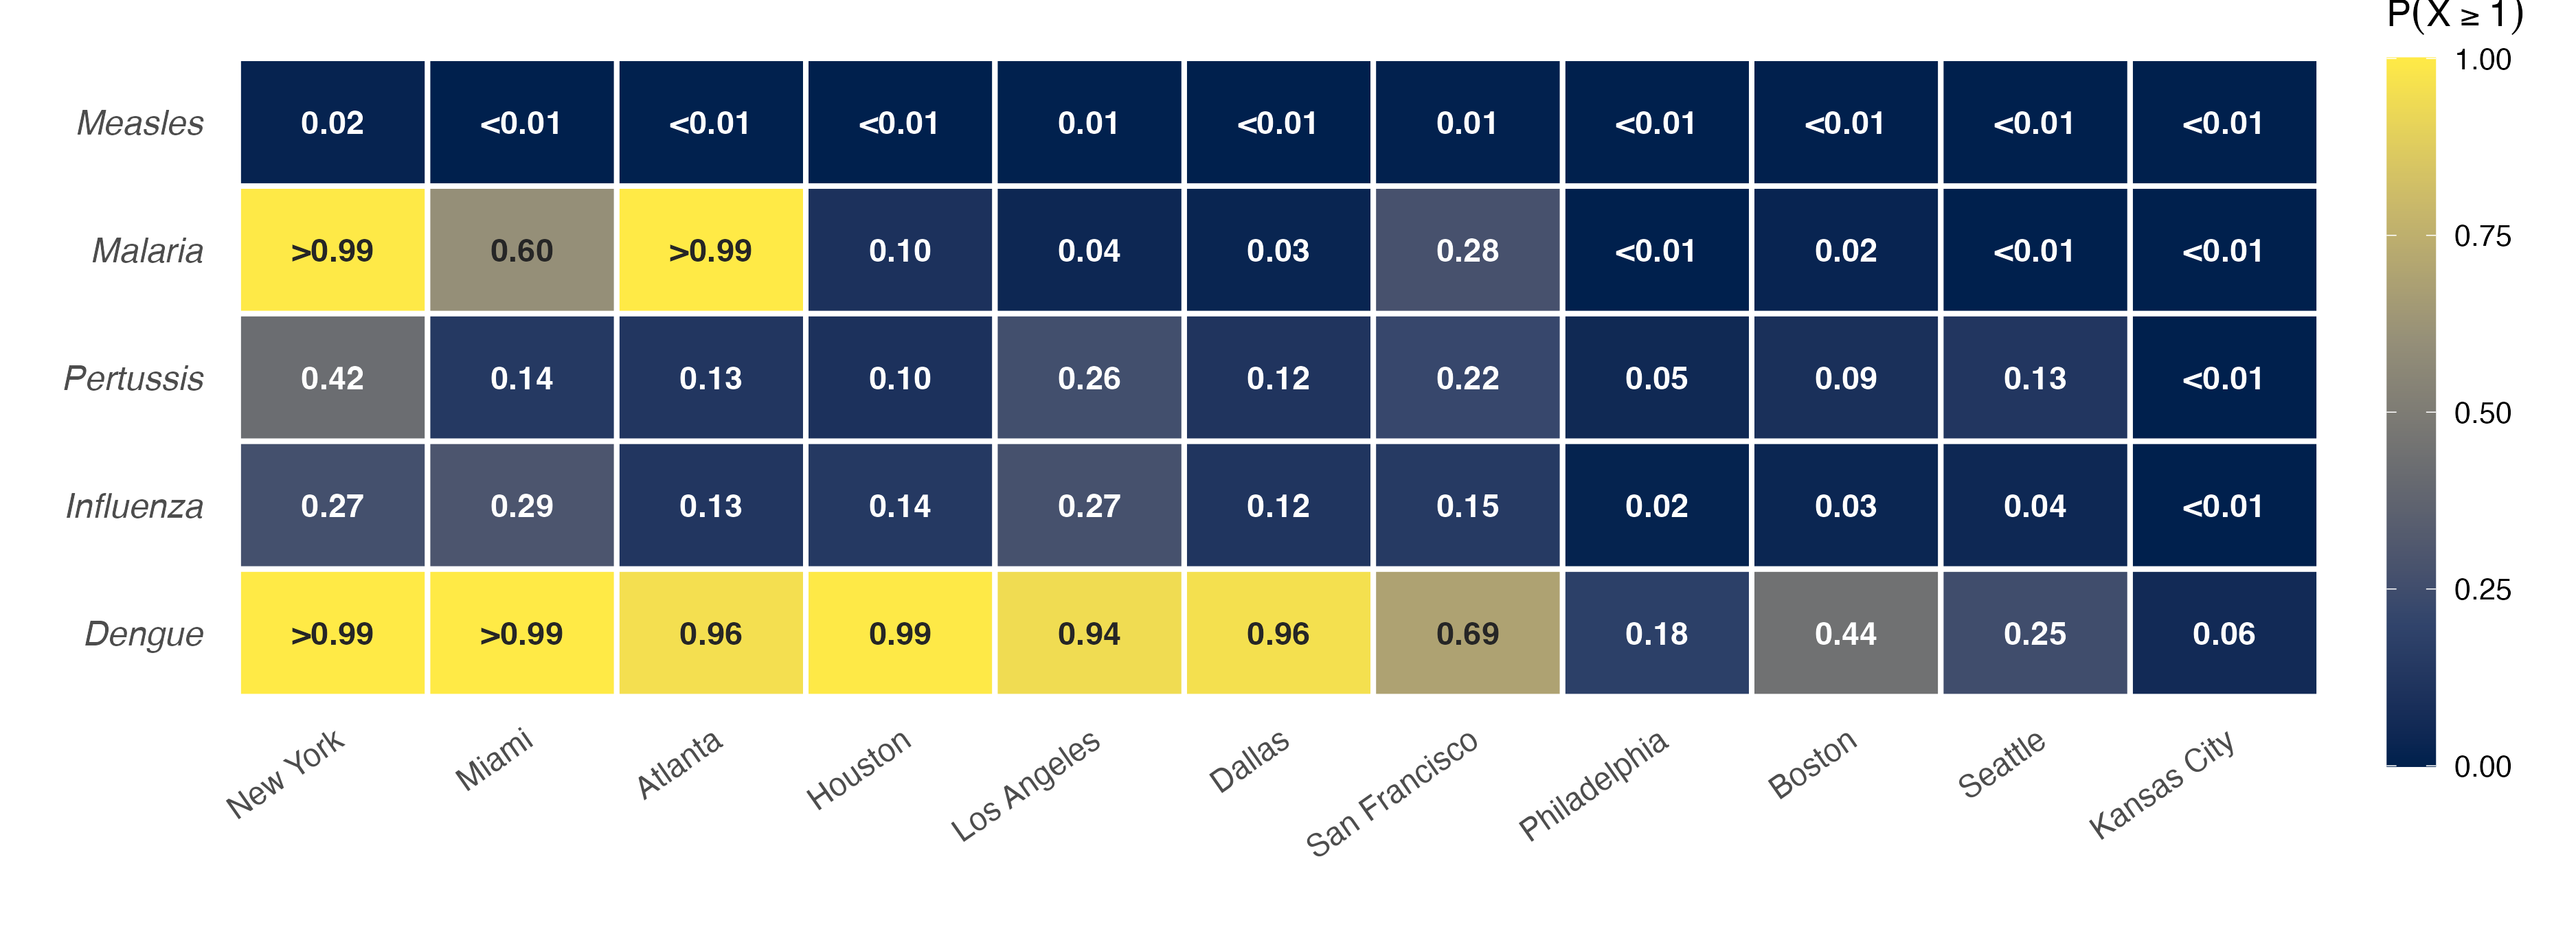
\includegraphics[width=\textwidth]{FigureS1.png}
  \caption*{\textbf{Figure S\arabic{suppfig}.}
    \textbf{Importation probability under the Baseline model (M1),
    June 2024 (no World Cup adjustment).}
    Same layout as Figure~\ref{fig:heatmap}. M1 represents the
    pre-tournament counterfactual: typical June travel volumes
    without the World Cup surge. Dengue $P(\geq 1) > 0.99$ is
    already present at Miami, New York, and Houston under baseline
    conditions, confirming that the World Cup amplifies but does
    not create the dengue importation threat.}
  \label{fig:s1}
\end{figure}

\newpage

% ---- Figure S2 ----------------------------------------------
\refstepcounter{suppfig}
\begin{figure}[htbp]
  \centering
  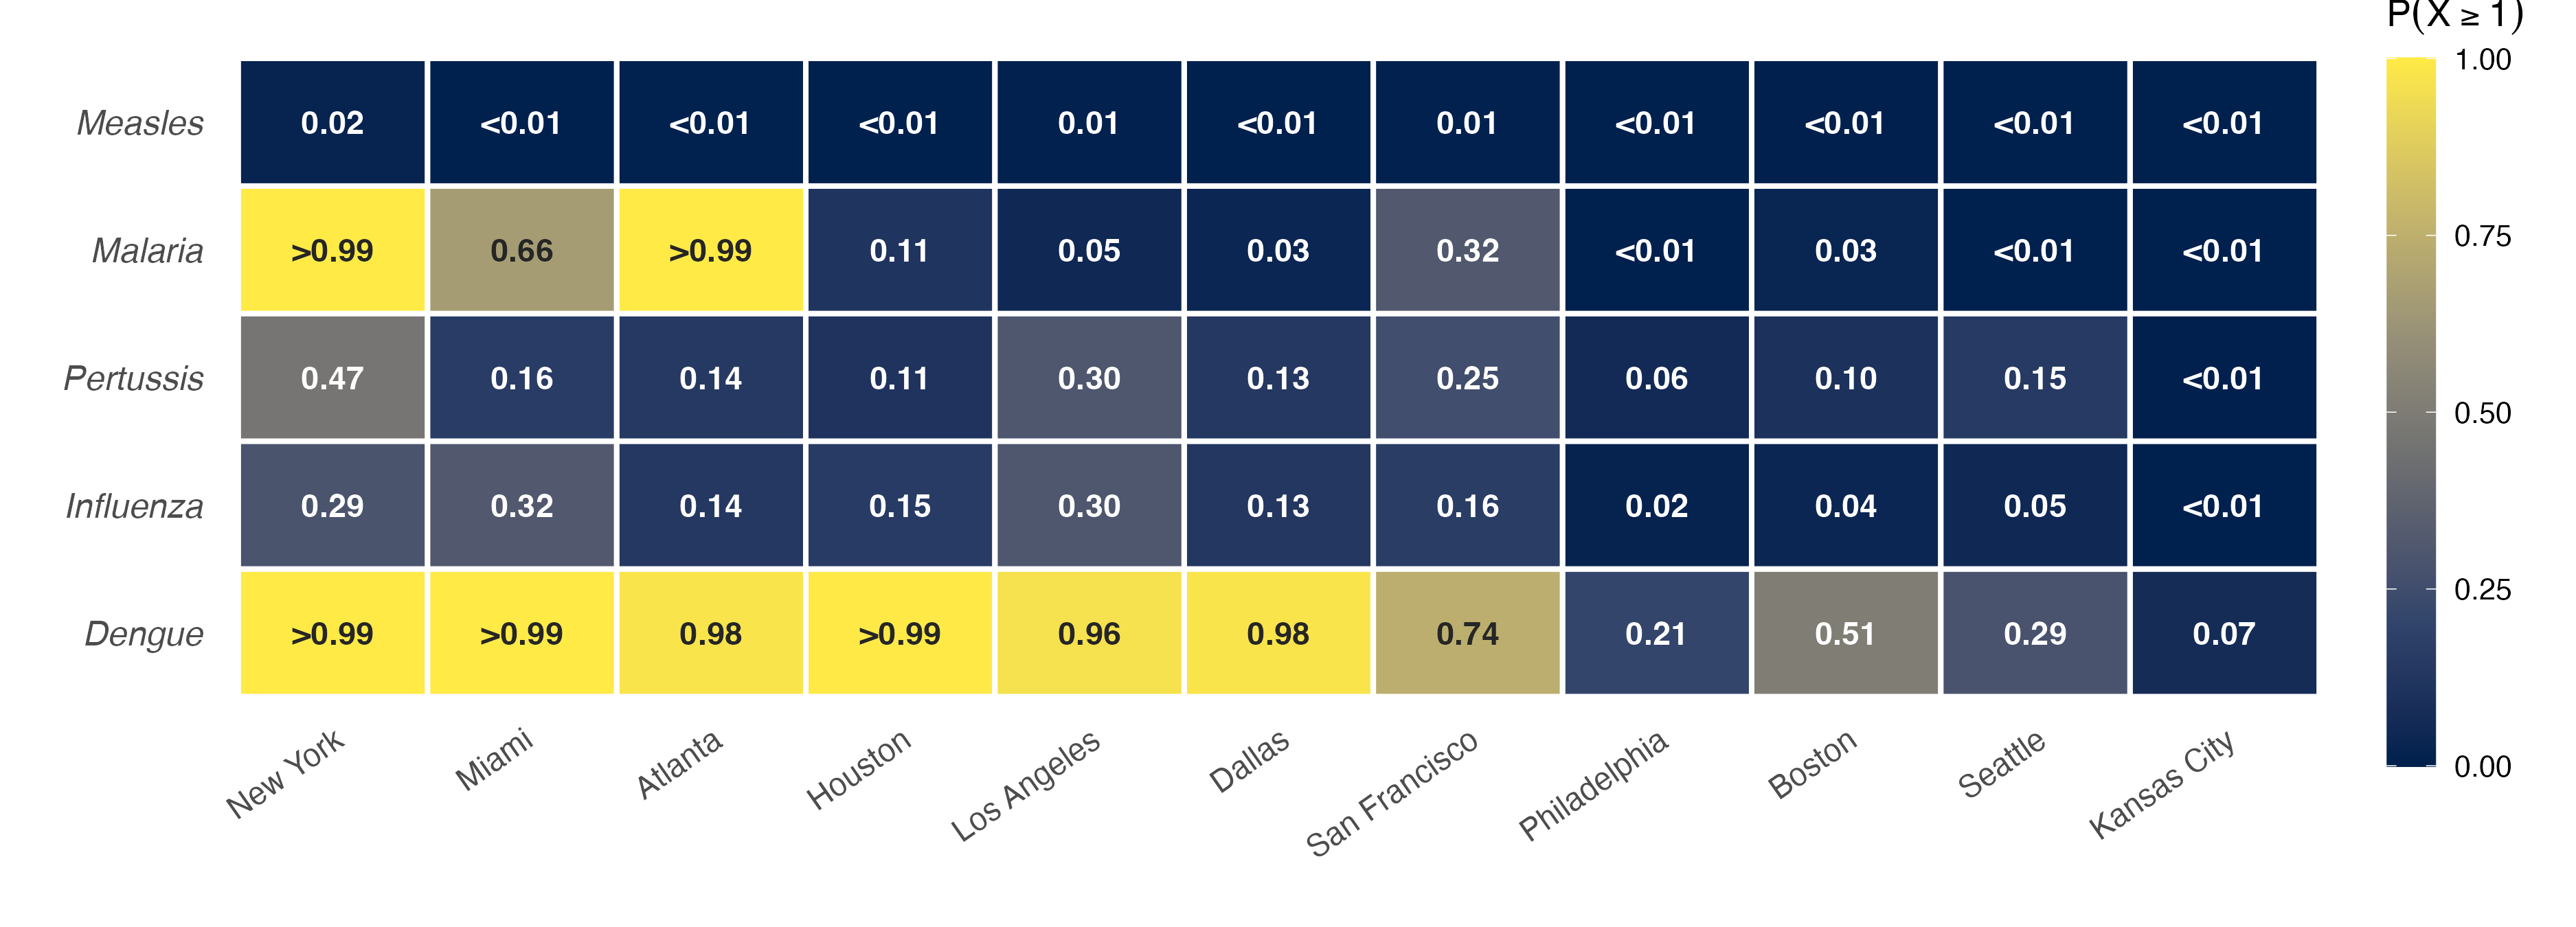
\includegraphics[width=\textwidth]{FigureS2.png}
  \caption*{\textbf{Figure S\arabic{suppfig}.}
    \textbf{Importation probability under the WC-adjusted model (M2),
    June 2026.}
    Same layout as Figure~\ref{fig:heatmap}. M2 applies World Cup
    growth factors to national arrivals but distributes all travel
    to US cities via T-100 routing fractions, including the fan
    increment for teams playing in Canada and Mexico. M2 values
    therefore represent a slight overestimate relative to M3 for
    US cities.}
  \label{fig:s2}
\end{figure}

\newpage

% ---- Figure S3 ----------------------------------------------
\refstepcounter{suppfig}
\begin{figure}[htbp]
  \centering
  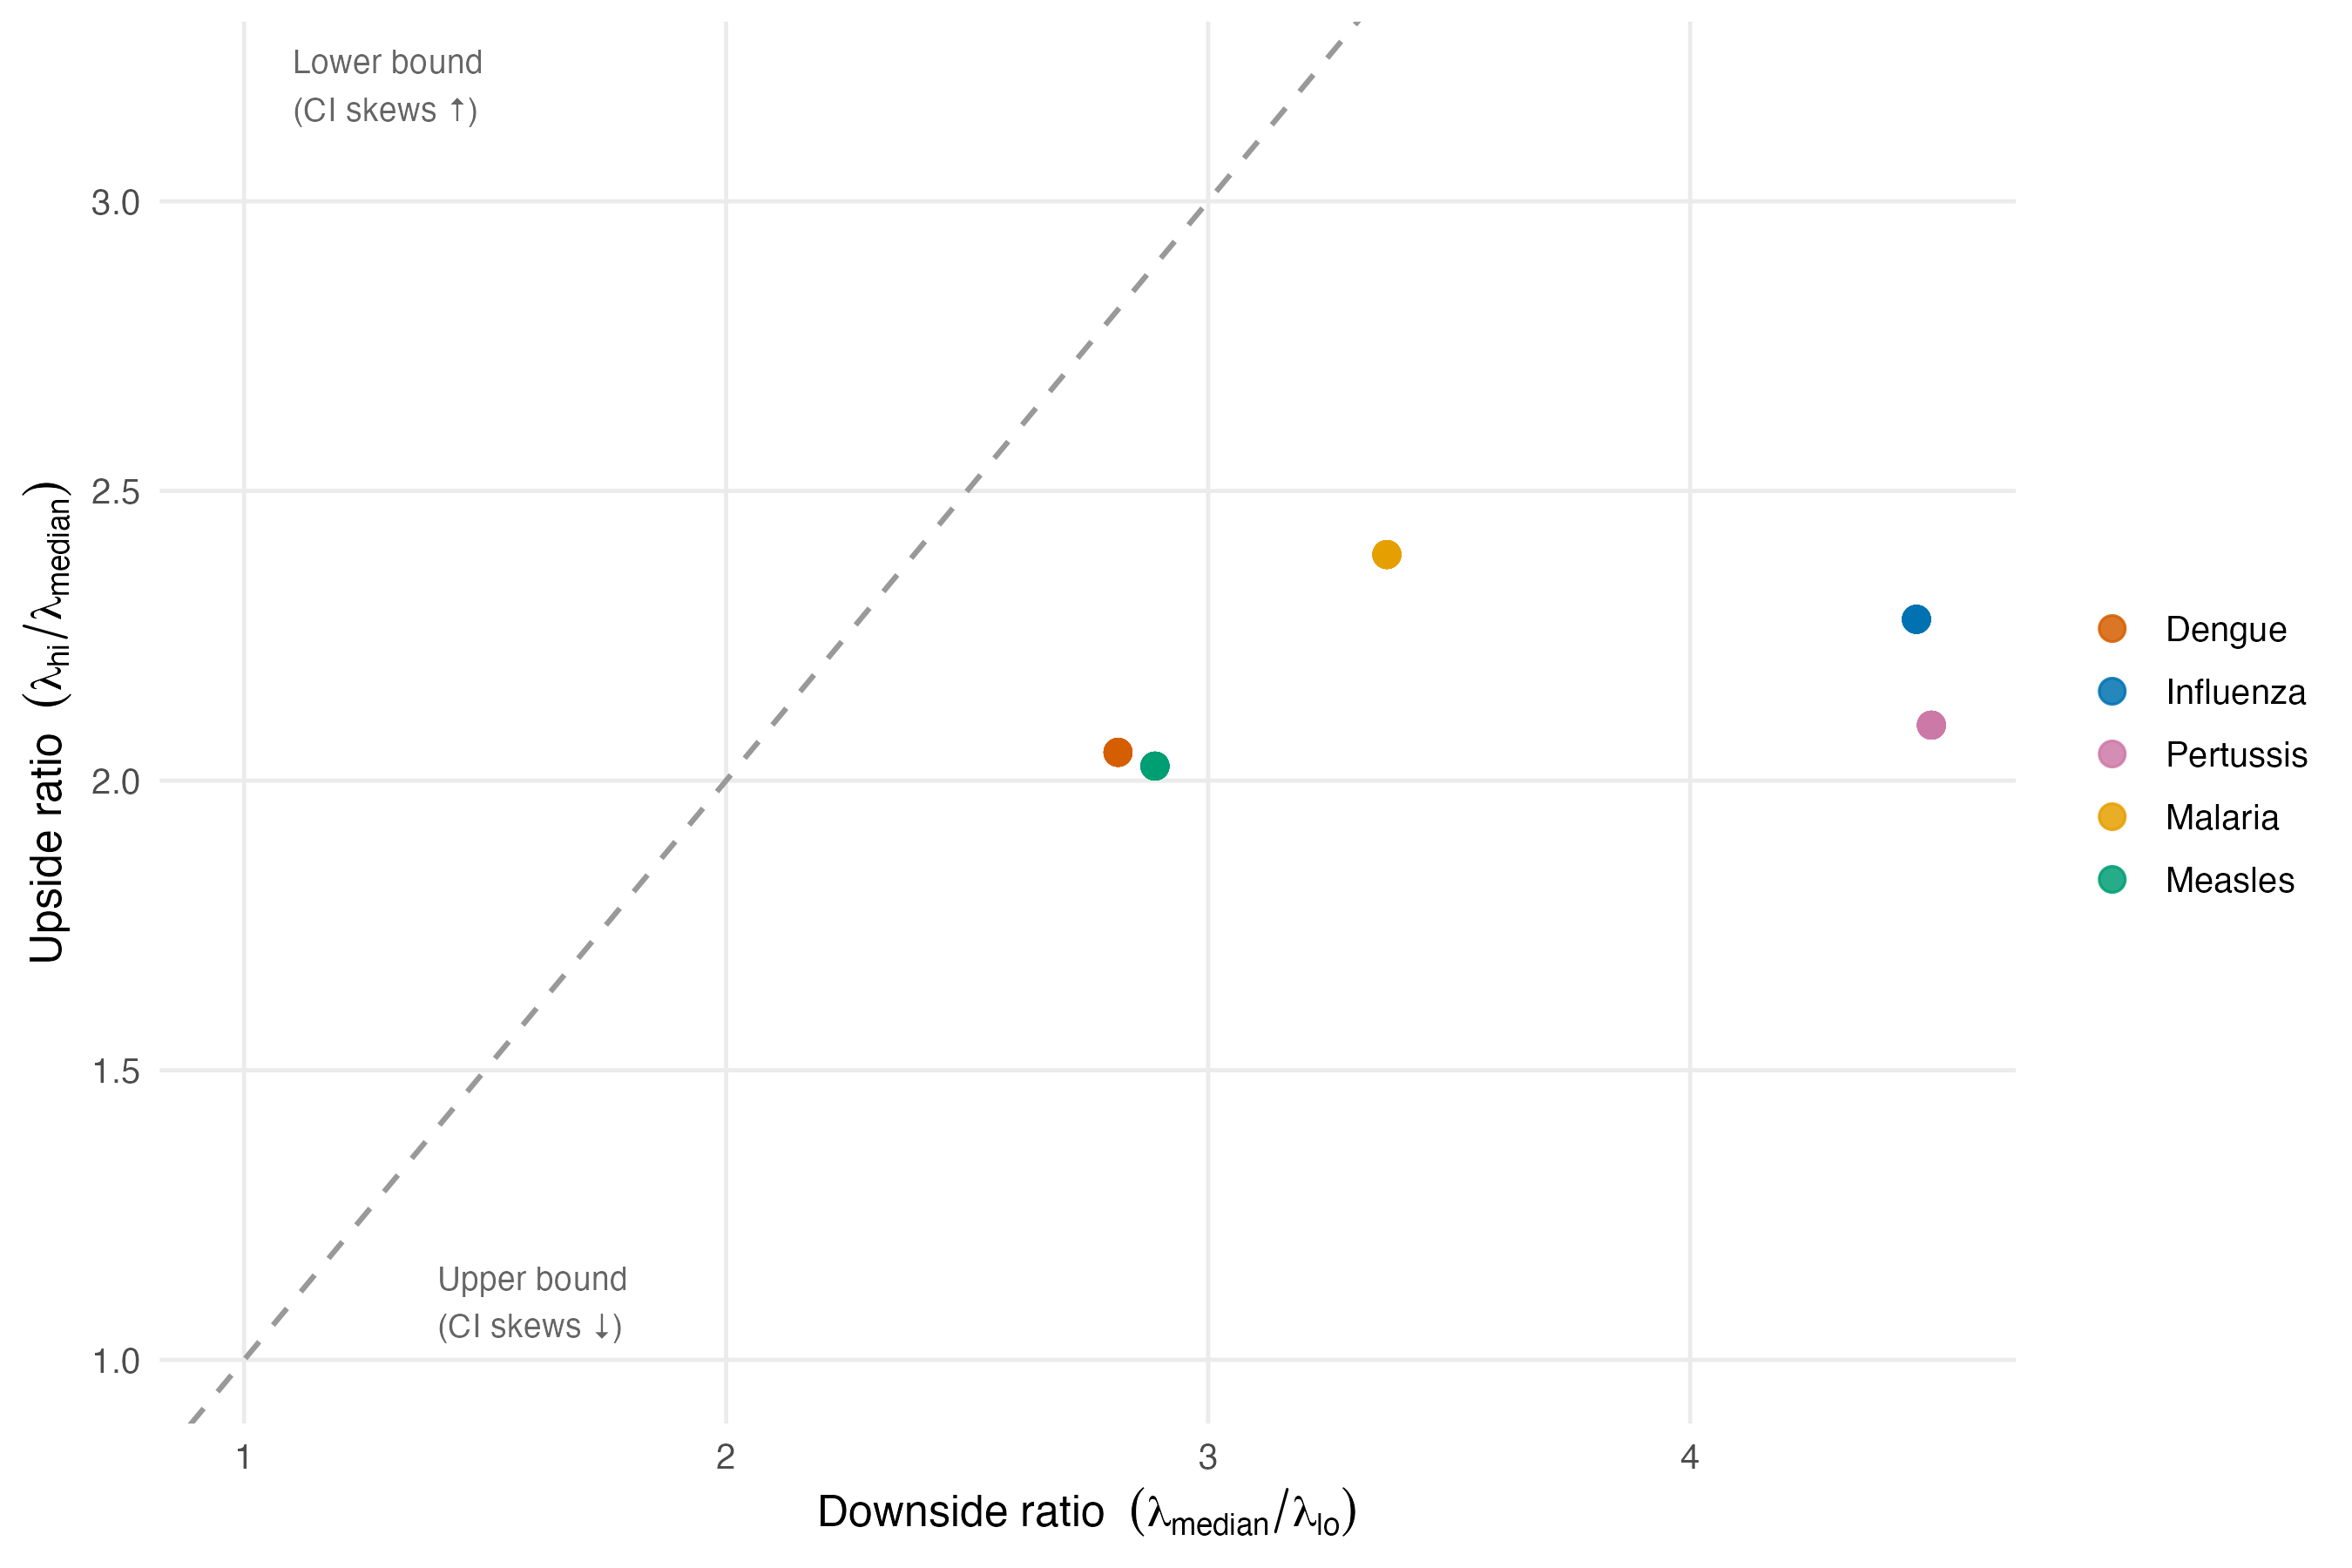
\includegraphics[width=0.85\textwidth]{FigureS3.png}
  \caption*{\textbf{Figure S\arabic{suppfig}.}
    \textbf{Direction of Monte Carlo uncertainty by disease.} Each point represents one disease--city combination. X-axis: downside ratio ($\lambda_\text{median}/\lambda_\text{lo}$), measuring how far the lower CI bound lies below the median. Y-axis: upside ratio ($\lambda_\text{hi}/\lambda_\text{median}$), measuring how far the upper CI bound lies above the median. Points above the diagonal have CIs that extend further upward; points below the diagonal have CIs that extend further downward, placing the central estimate closer to the upper plausible bound. All five diseases fall below the diagonal: uncertainty is asymmetrically larger on the  downside for every disease. Dengue and measles sit closest to the diagonal (downside ratio $\approx 2.8$), while malaria, influenza, and pertussis show larger downside ratios (4.3--4.8), indicating their medians are more conservative upper estimates.}
  \label{fig:s3}
\end{figure}

\newpage

% ---- Figure S4 ----------------------------------------------
\refstepcounter{suppfig}
\begin{figure}[htbp]
  \centering
  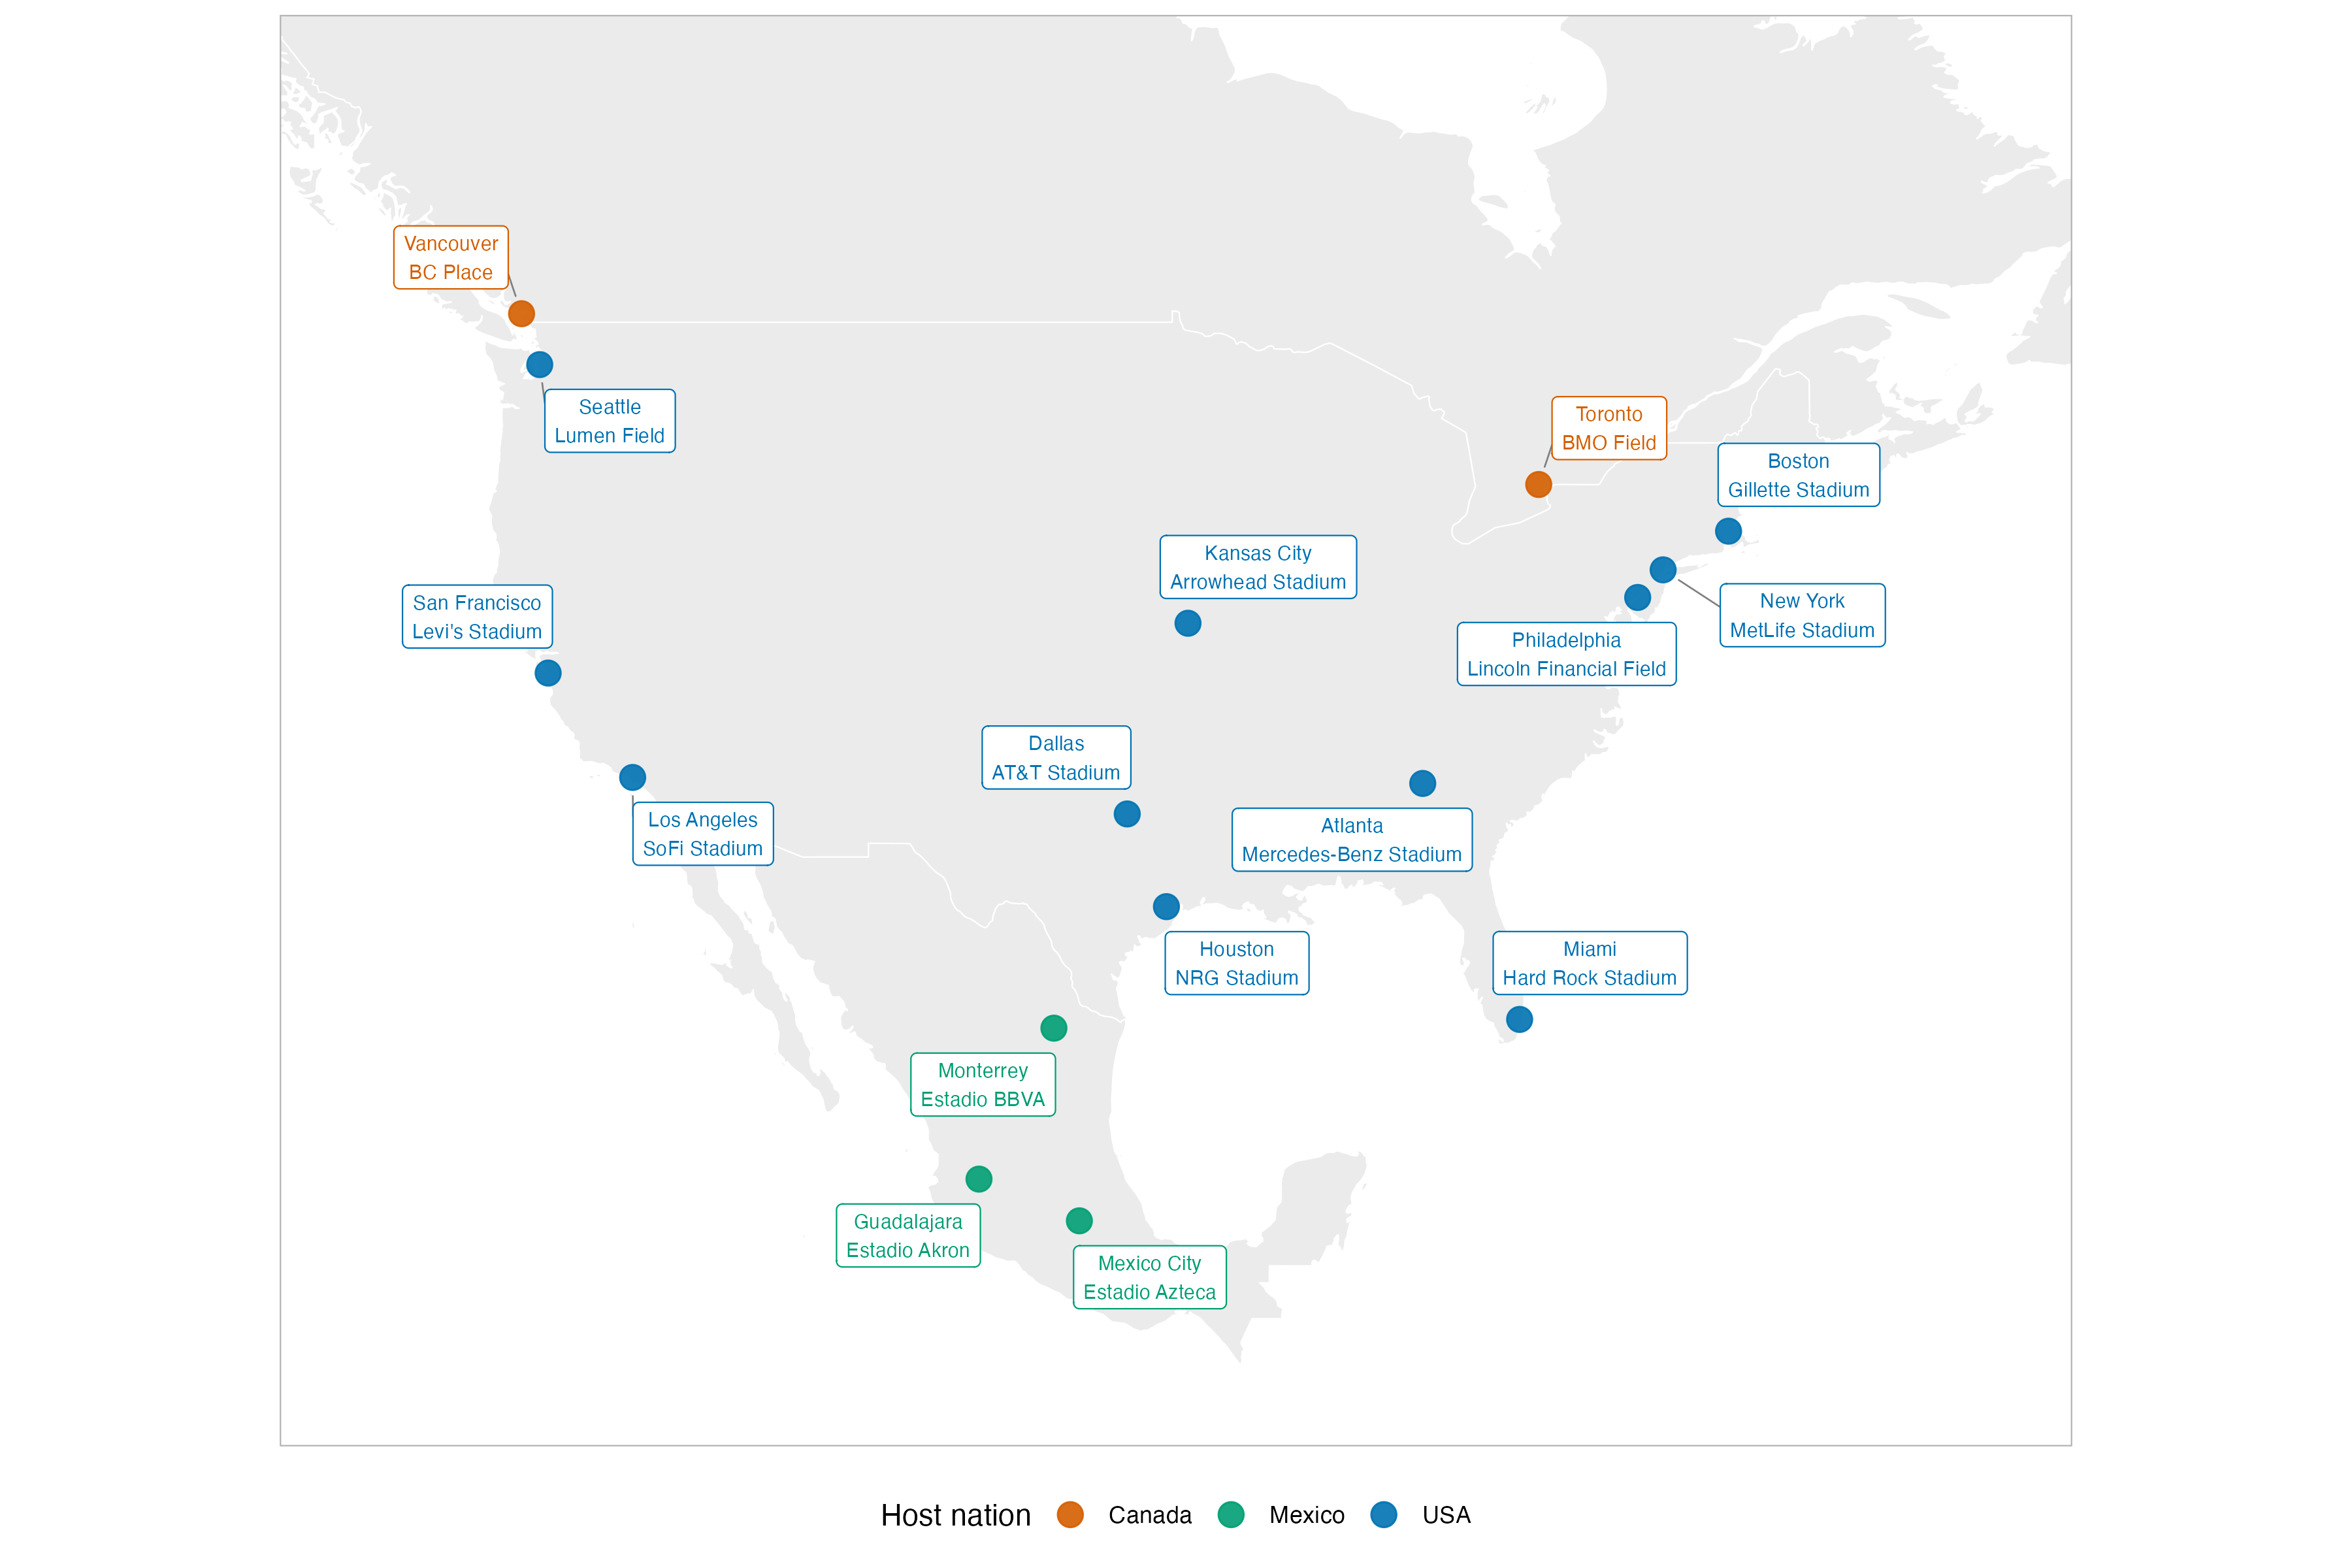
\includegraphics[width=\textwidth]{FigureS4.png}
  \caption*{\textbf{Figure S\arabic{suppfig}.}
    \textbf{Geographic distribution of the 16 FIFA World Cup 2026
    stadiums across the United States, Canada, and Mexico.}
    Colours indicate host nation. This analysis focuses on the 11
    US venues (blue); Canadian (Toronto, Vancouver) and Mexican
    (Mexico City, Monterrey, Guadalajara) venues are shown for
    context. The East Coast cluster (New York, Philadelphia, Boston)
    is the densest; Kansas City and Seattle are the most geographically
    isolated US venues.}
  \label{fig:s4}
\end{figure}

\newpage

% ---- Figure S5 ----------------------------------------------
\refstepcounter{suppfig}
\begin{figure}[htbp]
  \centering
  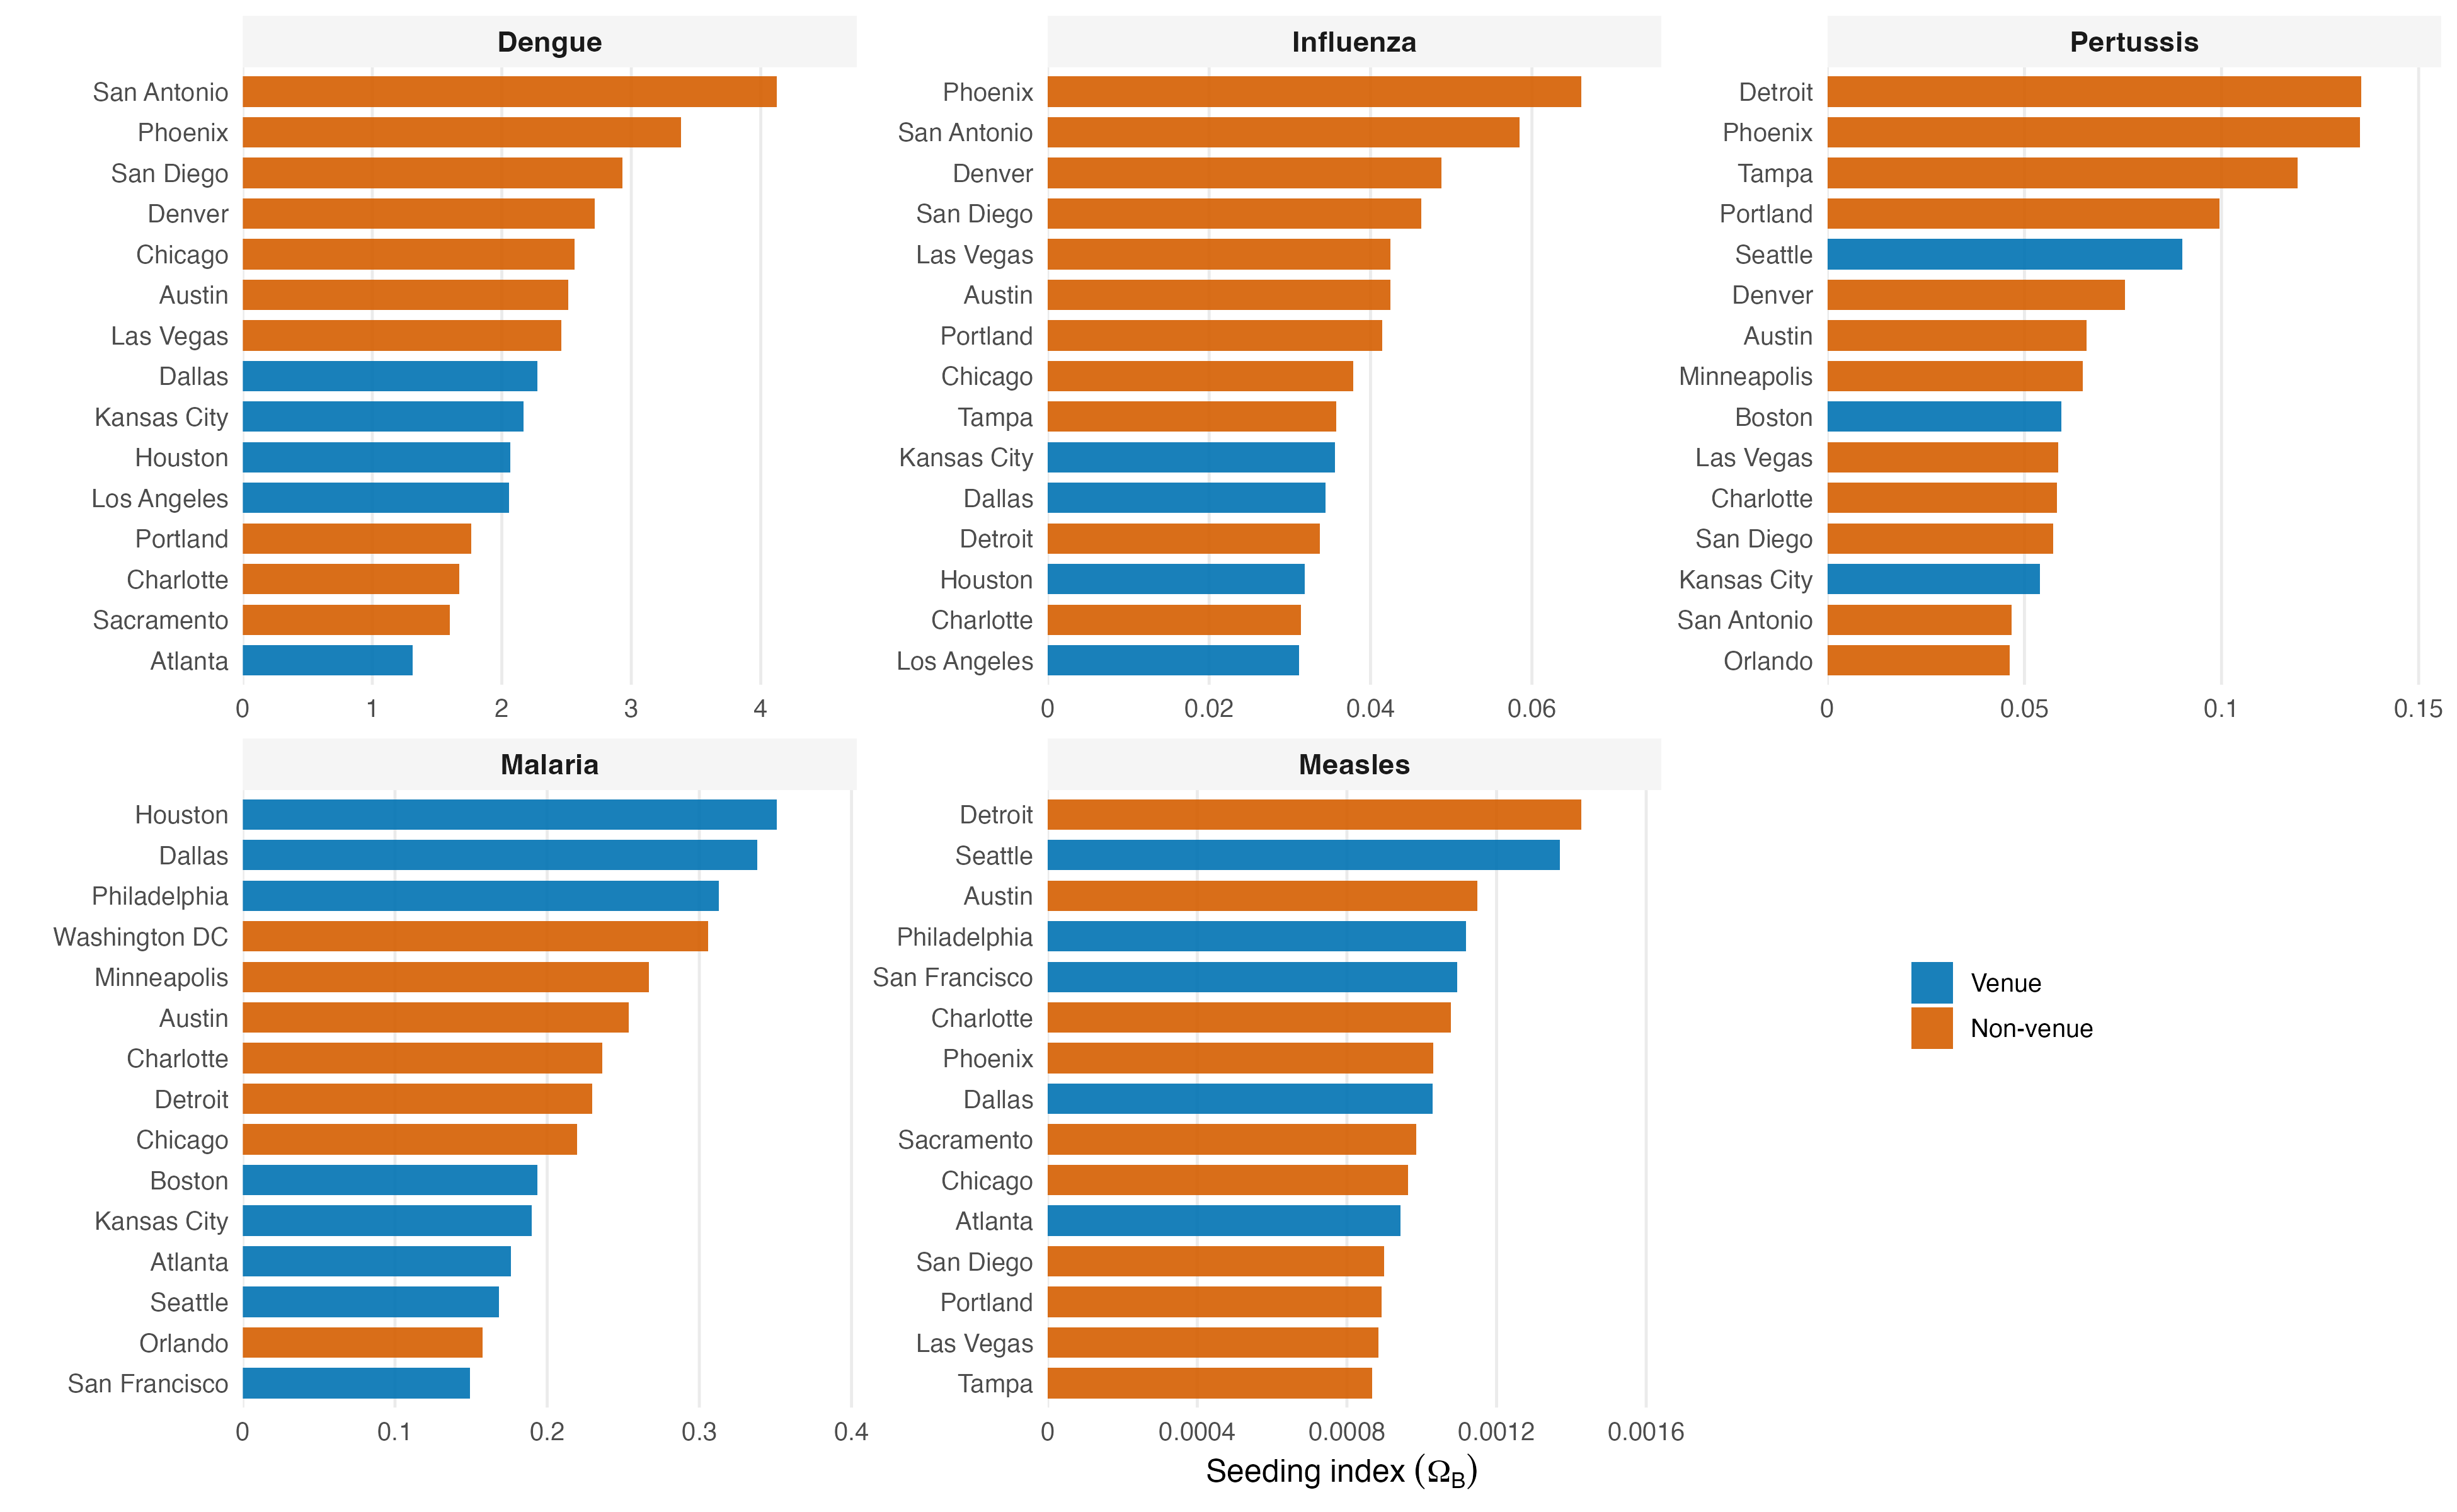
\includegraphics[width=\textwidth]{FigureS5.png}
 \caption*{\textbf{Figure S\arabic{suppfig}.}
    \textbf{Secondary seeding risk index ($\Omega^B$) for diaspora
    hub cities, by disease (Mechanism B).}
    Bars show the top 15 hub metropolitan areas per disease, ranked
    by $\Omega^B$ summed across all source countries and match venues,
    and colored by whether the hub is a World Cup host city or a
    non-host city. Hubs are the home cities to which diaspora members
    return after attending matches.}
  \label{fig:s5}
\end{figure}

\newpage

% ---- Figure S6 ----------------------------------------------
\refstepcounter{suppfig}
\begin{figure}[htbp]
  \centering
  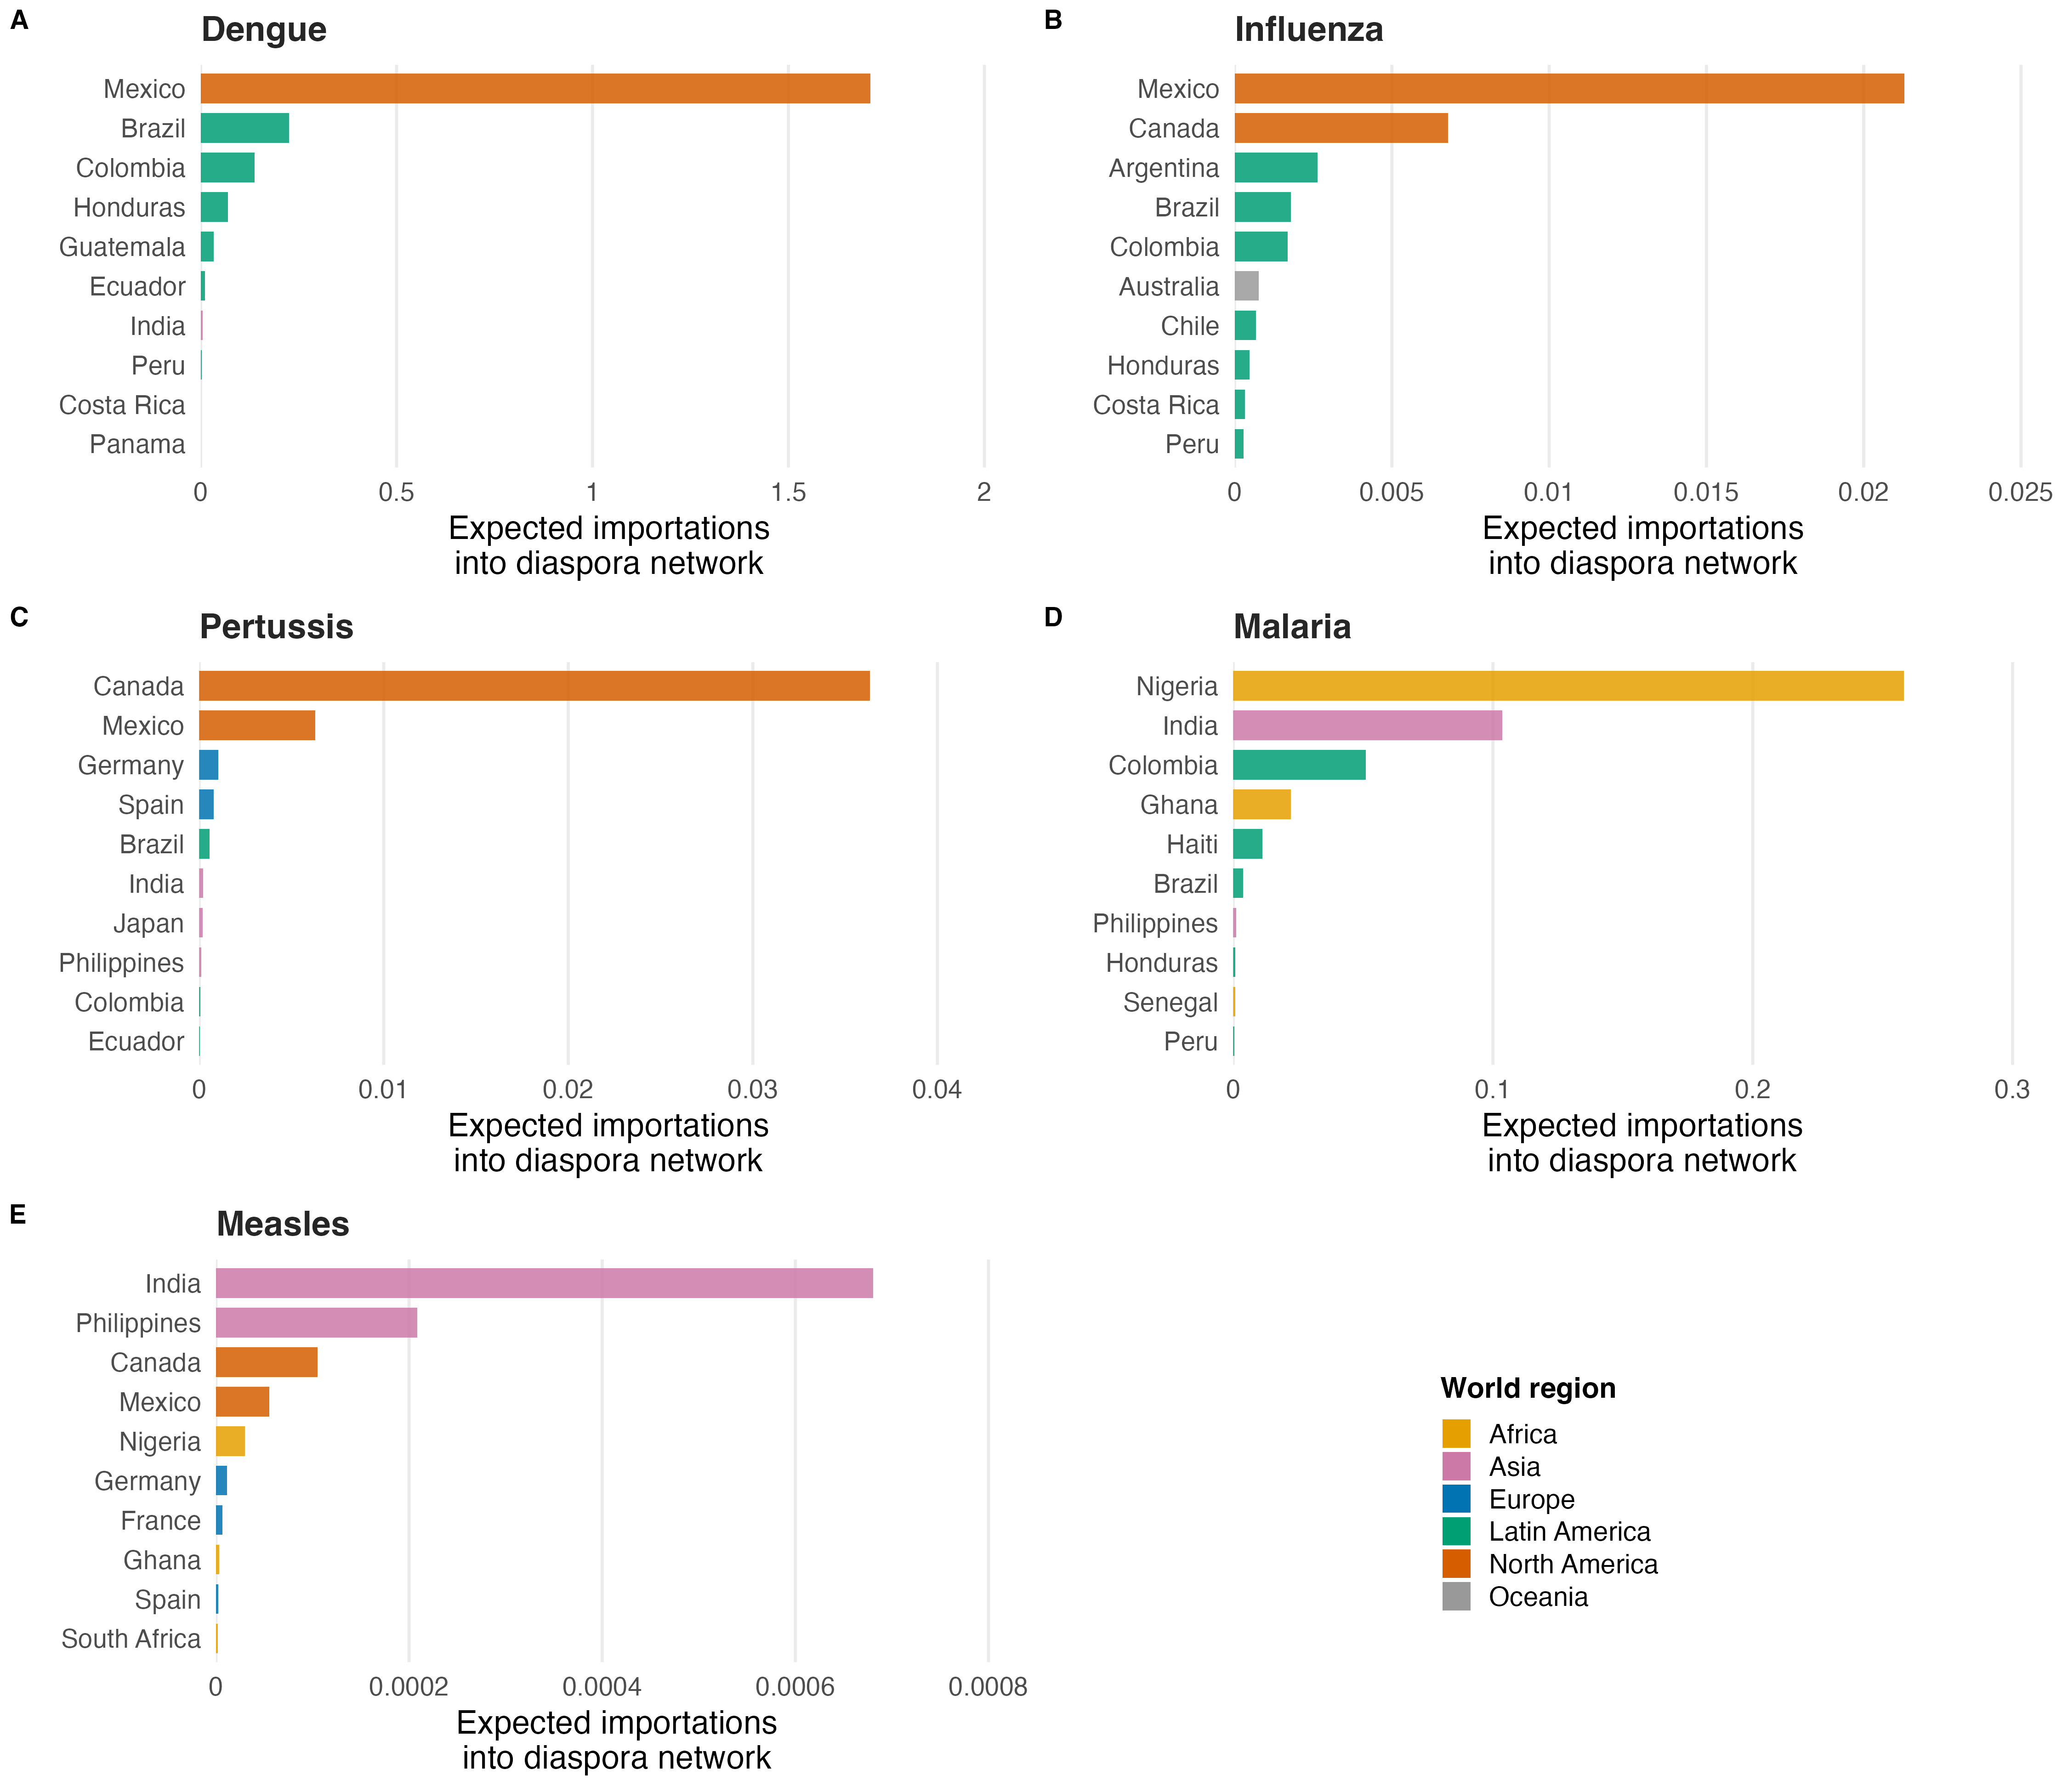
\includegraphics[width=\textwidth]{FigureS6.png}
  \caption*{\textbf{Figure S\arabic{suppfig}.}
    \textbf{Top 10 source-country contributors to diaspora-network
    importation intensity ($\Omega^A$) per disease.}
     Bars show $\Omega^A$ for each source country, summed across the
    11 host cities; colors denote world region (
Canada and Mexico
    grouped as North America). The corresponding
 raw-$\lambda$
    ranking is shown in Figure~\ref{fig:countries}.}
  \label{fig:s6}
\end{figure}

\newpage

% ---- Figure S7 ----------------------------------------------
\refstepcounter{suppfig}
\begin{figure}[htbp]
  \centering
  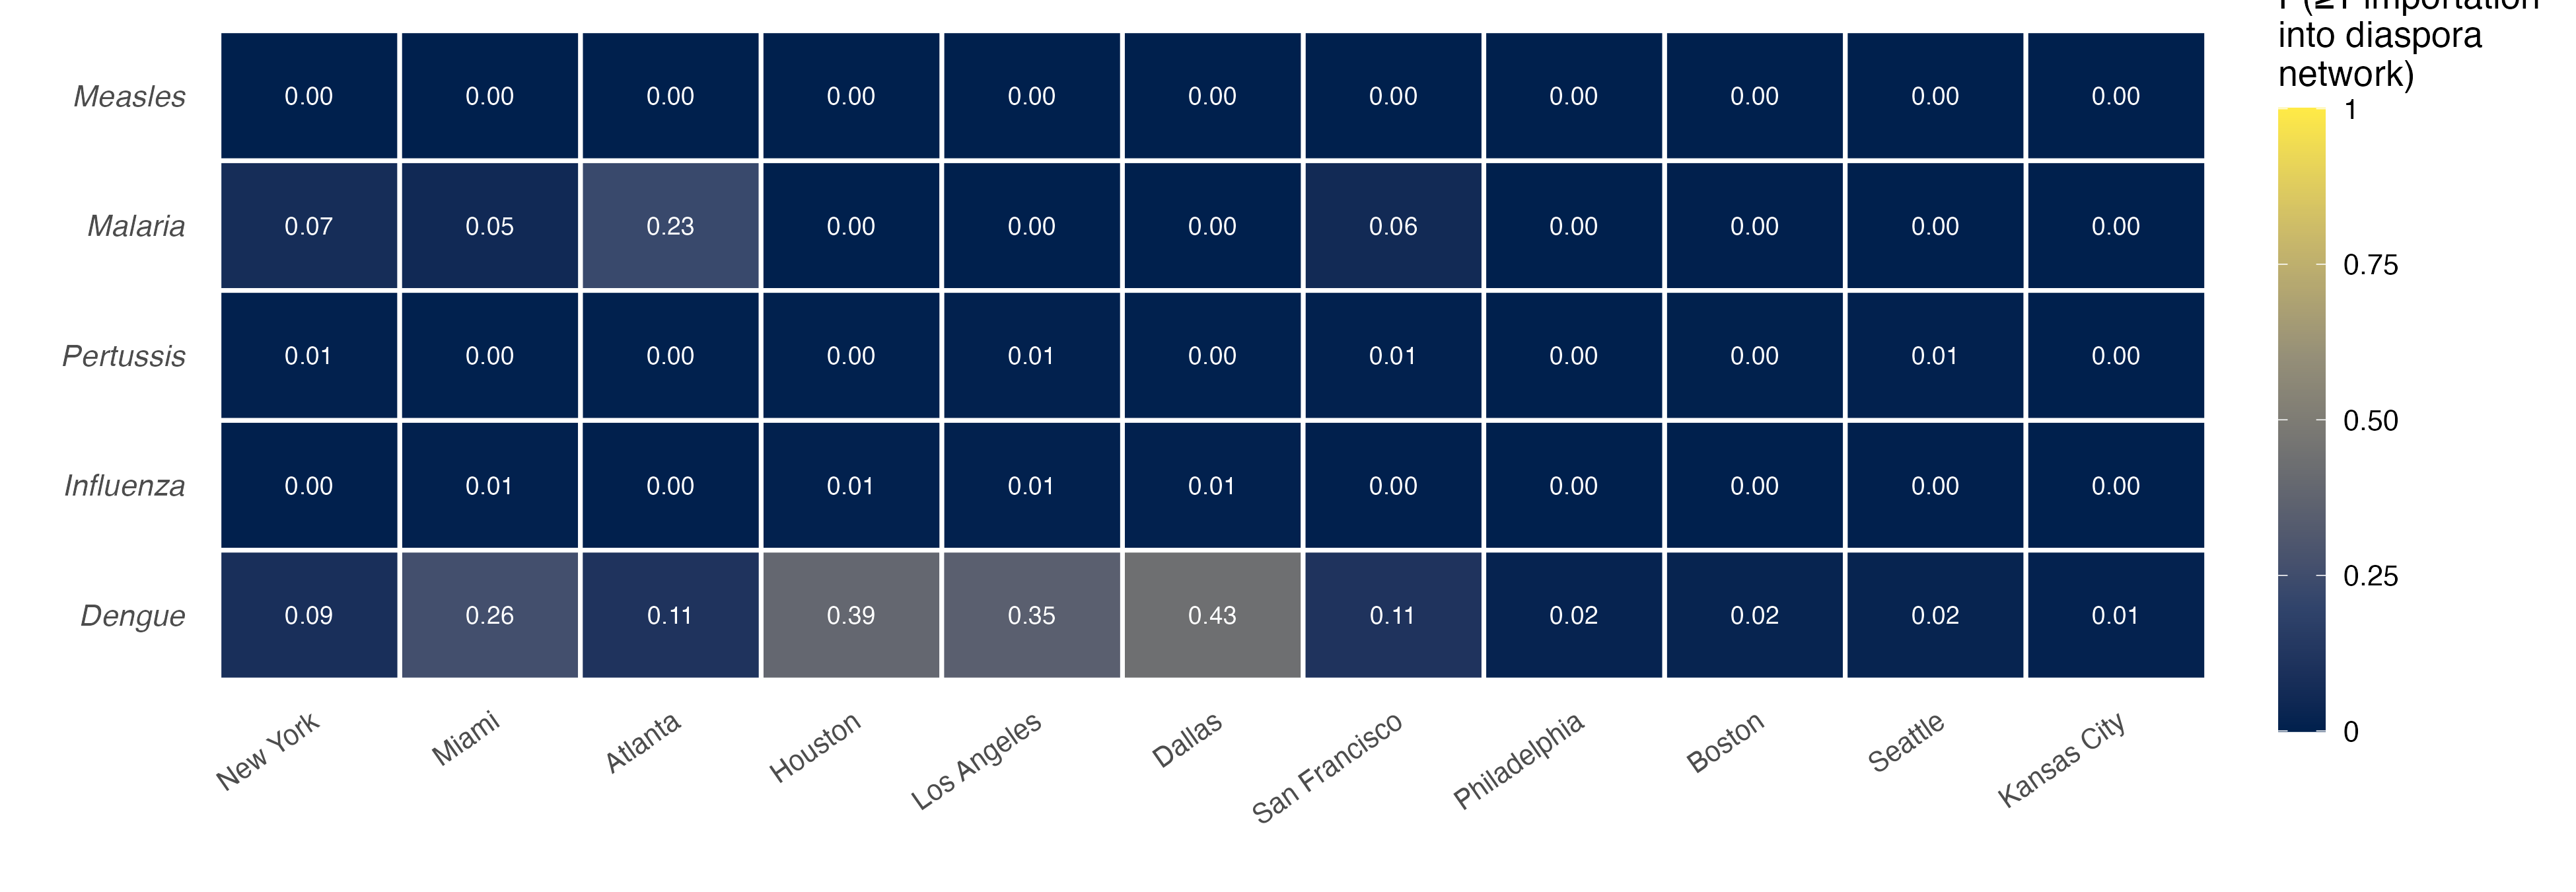
\includegraphics[width=\textwidth]{FigureS7.png}
  \caption*{\textbf{Figure S\arabic{suppfig}.}
    \textbf{Diaspora network importation probability ($P^A(\geq 1)$)
    for all five diseases at 11 US host cities.}
    Cells show $P^A(\geq 1)_{v,d}$, the probability that at least one
    imported case enters a co-national diaspora
network at each host
    city. The dengue and malaria rows correspond
 to Panel A of
    Figure~\ref{fig:diaspora} in the main text.}
  \label{fig:s7b}
\end{figure}

 % ---- Figure S8 ----------------------------------------------
\refstepcounter{suppfig}
 \begin{figure}[htbp]
   \centering
   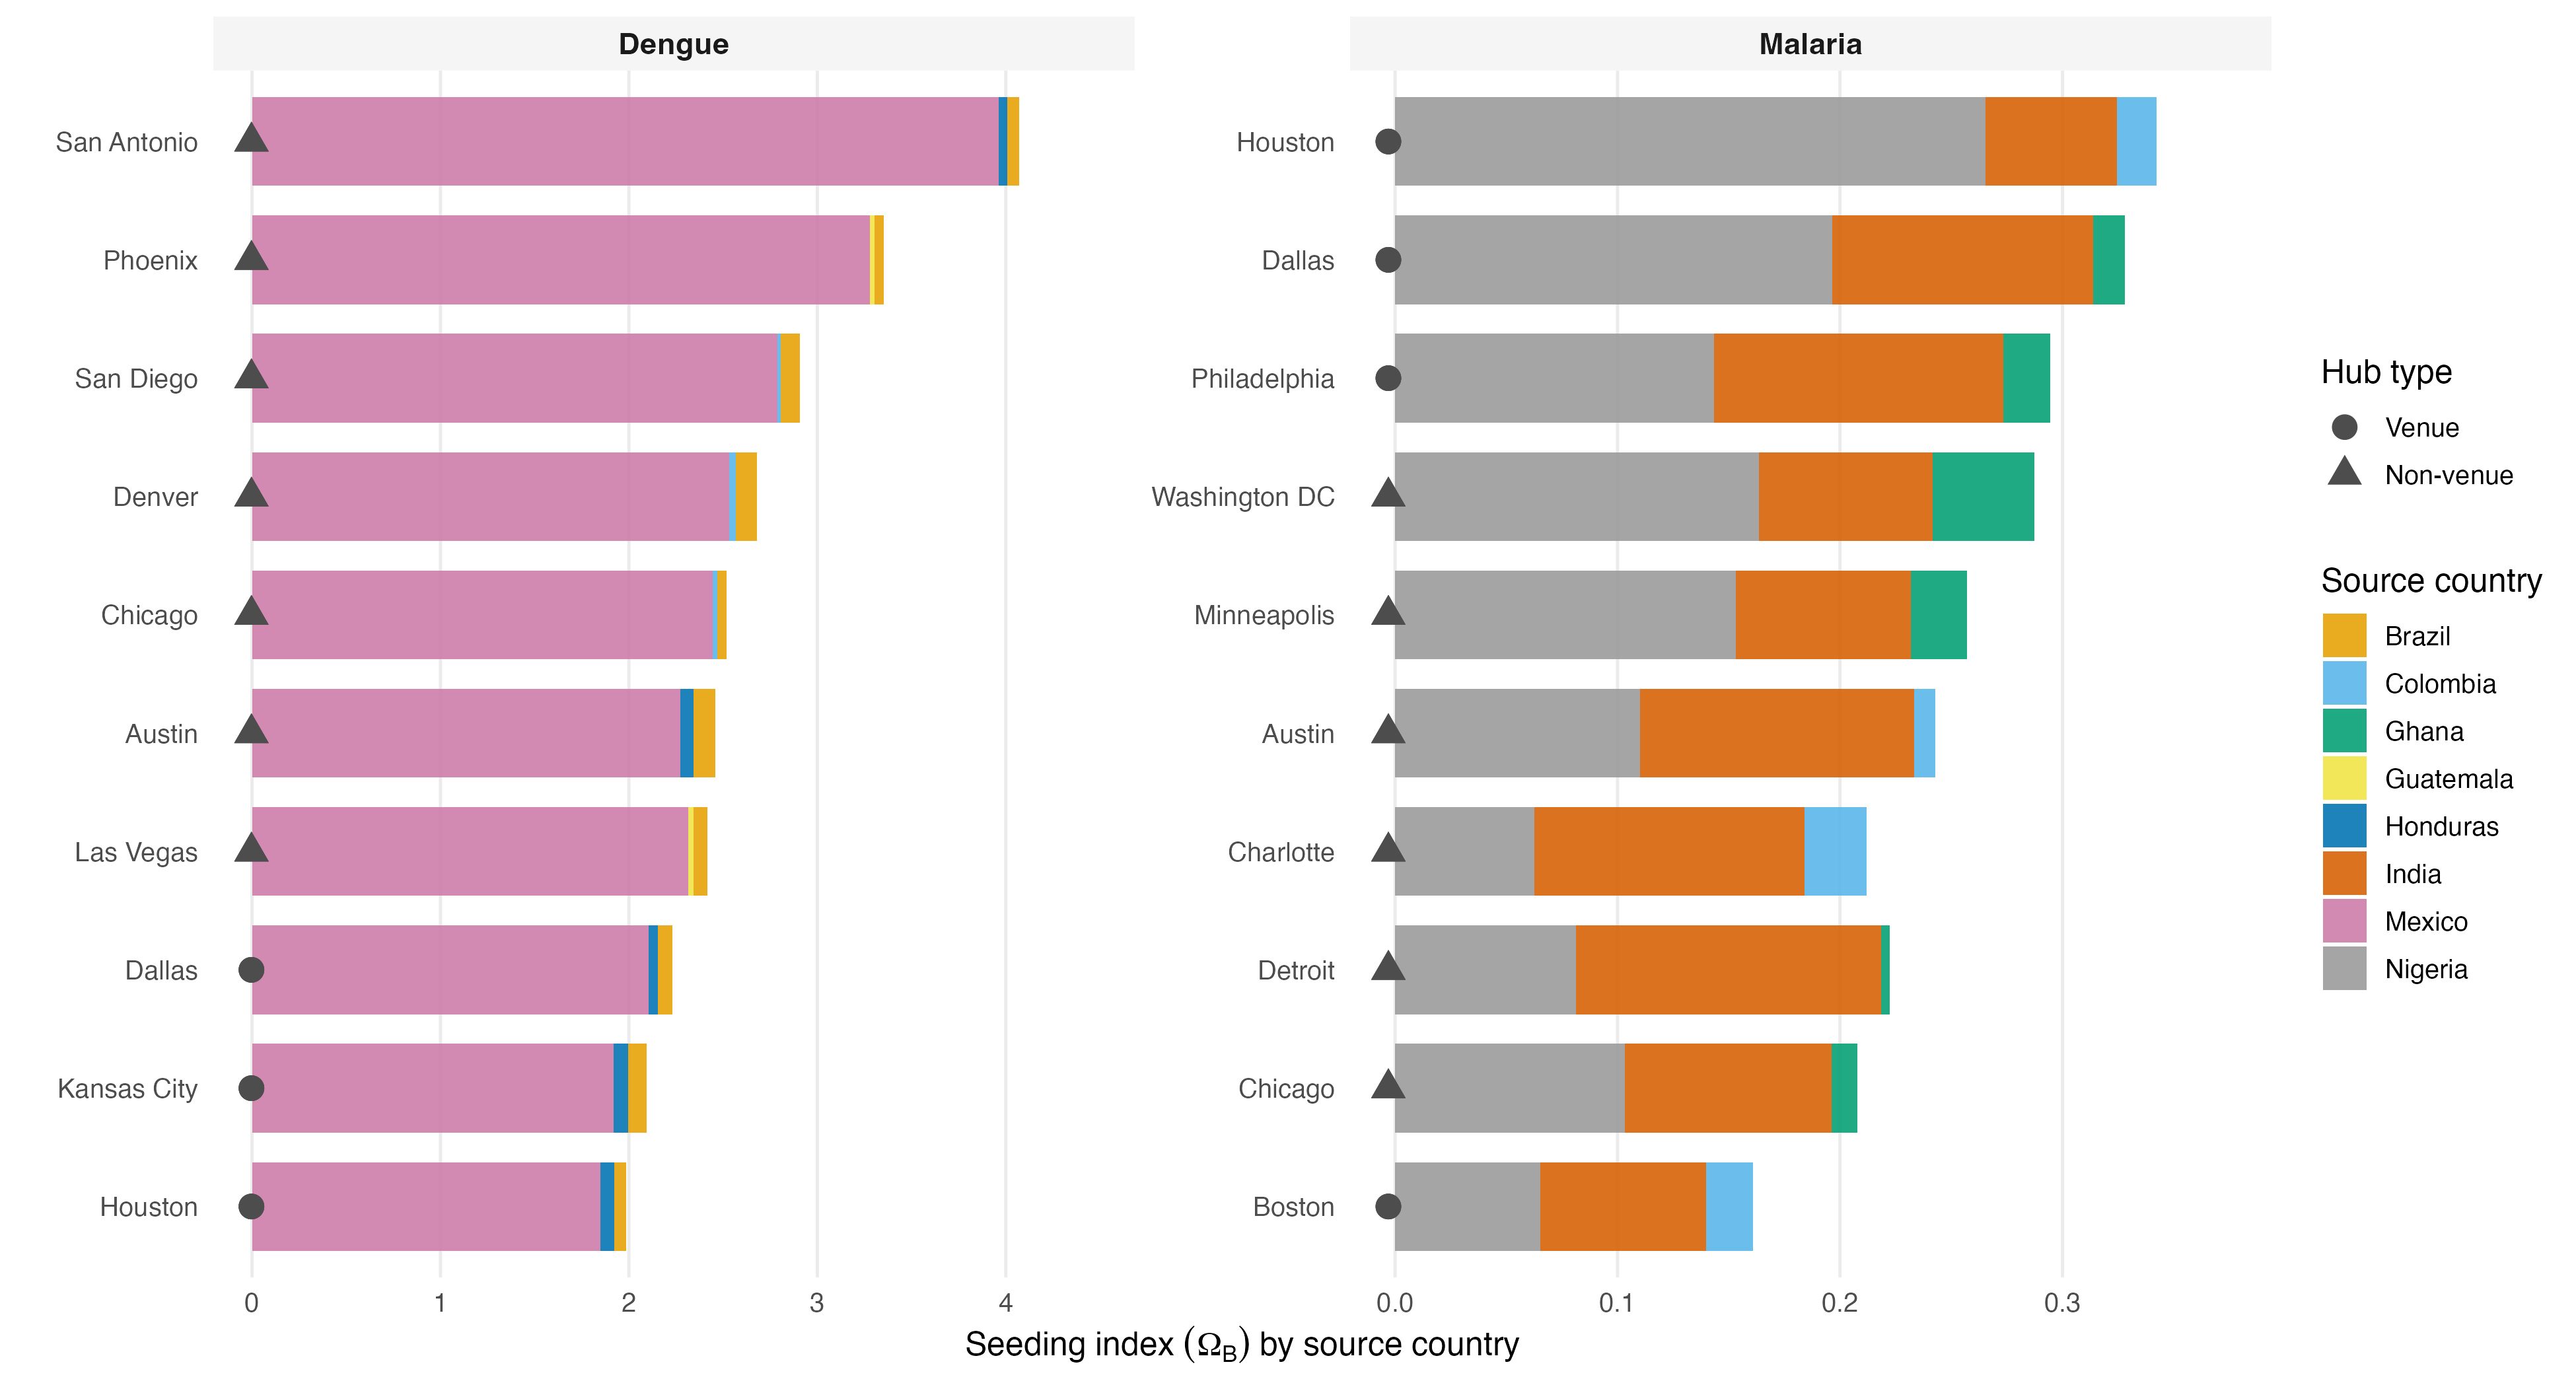
\includegraphics[width=\textwidth]{FigureS8.png}
   \caption*{\textbf{Figure S\arabic{suppfig}.} \textbf{Source-country contributions to Mechanism B secondary seeding index ($\Omega^B$) for dengue and malaria.}
      Bars show the three largest source-country contributions
  to
      $\Omega^B$ at each of the top 10 hub cities per disease,
  ranked
      by total $\Omega^B$. Dot shape distinguishes World Cup
  venue
      cities (circle) from non-venue metropolitan areas
  (triangle).
      For malaria, Nigerian and Indian diaspora communities
  drive
      secondary seeding at all top hubs; non-venue cities
      (Washington, DC; Minneapolis; Austin; Charlotte; Detroit;
  and
      Chicago) rank alongside host cities (Houston, Dallas, and
      Philadelphia) because of their large co-national diaspora
      concentrations. For dengue, Mexican diaspora communities
      dominate, with non-venue hubs outranking most host
  cities.}
    \label{fig:s8}
  \end{figure}

\end{document}
